\documentclass[aspectratio=43]{beamer}

% ──────────────────────────────────────────────────────────────────────────────
%                         BEAMER DOCUMENT PREAMBLE
% ──────────────────────────────────────────────────────────────────────────────

% ──────────────────────────────────────────────────────────────────────────────
% 0. BASICS/UTILITY
% ──────────────────────────────────────────────────────────────────────────────
\usepackage{amsmath}
\usepackage{extarrows}
\usepackage{pgffor}
\usepackage{array}
\usepackage{graphicx}
\usepackage[svgnames]{xcolor}
\usepackage[percent]{overpic}
\usepackage[export]{adjustbox}
\usepackage{xparse}
\usepackage[backend=biber]{biblatex}
\DeclareMathOperator*{\argmax}{arg\,max}
\DeclareMathOperator*{\argmin}{arg\,min}

% ──────────────────────────────────────────────────────────────────────────────
% 1. THEME & FONT THEME
% ──────────────────────────────────────────────────────────────────────────────
\usetheme{default}                  % Base beamer theme
\usecolortheme{default}             % Base color theme
\usefonttheme{structurebold}        % Bold structural fonts

% ──────────────────────────────────────────────────────────────────────────────
% 2. PAGE MARGINS & FRAME TITLE LAYOUT
% ──────────────────────────────────────────────────────────────────────────────
\setbeamersize{text margin left=1.5cm, text margin right=1.5cm}
\setbeamertemplate{frametitle}[default][%
  left,                              % Align title to the left
  leftskip=0.5cm,                    % Indent from left edge
  sep=0.5cm                          % Space between title and content
]

% ──────────────────────────────────────────────────────────────────────────────
% 3. COLOR DEFINITIONS
% ──────────────────────────────────────────────────────────────────────────────
\definecolor{primaryblue}{RGB}{70, 130, 180}  % Accent blue
\definecolor{primaryred}{RGB}{229, 57, 53}  % Accent red
\definecolor{lightgray}{RGB}{245, 245, 245}   % Light background gray
\definecolor{darkgray}{RGB}{80, 80, 80}       % Dark text gray
\definecolor{bluegrey}{RGB}{120, 144, 156}     % Caption label color
\definecolor{grey}{RGB}{158, 158, 158}          % Caption text color
\definecolor{cquoteframe}{RGB}{30,60,100}          % Quote box frame
\definecolor{cquoteback}{RGB}{240,245,252}          % Quote box background fill

% ──────────────────────────────────────────────────────────────────────────────
% 4. BEAMER COLOR THEMES
% ──────────────────────────────────────────────────────────────────────────────
\setbeamercolor{structure}{fg=primaryblue}    % Structural elements
\setbeamercolor{frametitle}{fg=primaryblue}   % Frame title

% Block styles
\setbeamercolor{block title}{bg=primaryblue, fg=white}
\setbeamercolor{block body}{bg=lightgray}
\setbeamercolor{block title alerted}{bg=red!80, fg=white}
\setbeamercolor{block body alerted}{bg=red!10}
\setbeamercolor{block title example}{bg=green!80, fg=white}
\setbeamercolor{block body example}{bg=green!10}

% ──────────────────────────────────────────────────────────────────────────────
% 5. NAVIGATION & FOOTLINE
% ──────────────────────────────────────────────────────────────────────────────
\setbeamertemplate{navigation symbols}{}      % Remove navigation symbols

\setbeamertemplate{footline}{%             % Custom footline with page numbers
  \hfill%
  \usebeamercolor[fg]{page number in head/foot}%
  \usebeamerfont{page number in head/foot}%
  \insertframenumber\,/\,\inserttotalframenumber\kern1em\vskip2pt%
}

% ──────────────────────────────────────────────────────────────────────────────
% 6. LIST ITEM ICONS
% ──────────────────────────────────────────────────────────────────────────────
\setbeamertemplate{itemize items}[circle]
\setbeamertemplate{enumerate items}[default]

% ──────────────────────────────────────────────────────────────────────────────
% 7. CUSTOM HIGHLIGHT COMMAND
% ──────────────────────────────────────────────────────────────────────────────
\newcommand{\bhighlight}[1]{\textcolor{primaryblue}{#1}}
\newcommand{\rhighlight}[1]{\textcolor{primaryred}{#1}}

% ──────────────────────────────────────────────────────────────────────────────
% 8. SENTIMENT COLORS & COMMANDS
% ──────────────────────────────────────────────────────────────────────────────
\definecolor{BeamerNegativeRed}{rgb}{0.8,0.1,0.1}
\definecolor{BeamerPositiveGreen}{rgb}{0.05,0.5,0.05}
\definecolor{BeamerNeutralBlue}{rgb}{0.0,0.45,0.85}

\setbeamercolor{negative text}{fg=BeamerNegativeRed}
\setbeamercolor{positive text}{fg=BeamerPositiveGreen}
\setbeamercolor{neutral text}{fg=BeamerNeutralBlue}

\newcommand{\negative}[1]{{\usebeamercolor[fg]{negative text}#1}}
\newcommand{\positive}[1]{{\usebeamercolor[fg]{positive text}#1}}
\newcommand{\neutral}[1]{{\usebeamercolor[fg]{neutral text}#1}}

% ──────────────────────────────────────────────────────────────────────────────
% 9. CAPTION SETTINGS
% ──────────────────────────────────────────────────────────────────────────────
\usepackage{caption}
\setbeamerfont{caption}{size=\scriptsize}     % Smaller caption font
\setbeamertemplate{caption}[numbered]          % Number figures/tables
\newcommand{\gcite}[1]{\textcolor{grey}{#1}}

\newcommand{\insetcaption}[3][]{%
  \begin{overpic}[#1]{#2}
    \put(50,3){\makebox(0,0)[c]{\color{gray}\tiny #3}}
  \end{overpic}%
}
% ──────────────────────────────────────────────────────────────────────────────
% 10. FONTS & MATH SETUP
% ──────────────────────────────────────────────────────────────────────────────
\usepackage{fontspec}                           % XeLaTeX or LuaLaTeX font support
\setsansfont{Linux Biolinum}                    % Primary sans-serif font
\usepackage{unicode-math}                       % Unicode math support
\setmathfont{Libertinus Math}                   % Math font

% ──────────────────────────────────────────────────────────────────────────────
% 11. QUOTES
% ──────────────────────────────────────────────────────────────────────────────
\usepackage[most]{tcolorbox}
\tcbset{
  quote/.style={
      colback=cquoteback,    % fill color
      colframe=cquoteframe, % border color
      fonttitle=\bfseries,
      boxrule=0.8pt,
      arc=4pt,              % corner radius
      boxsep=8pt,           % inner padding
      left=4pt, right=4pt, top=4pt, bottom=4pt,
      width=0.75\textwidth, % box width
      center title,
      before skip=1em,
      after skip=1em
    }
}
\newenvironment{cquote}
{\begin{center}%
    \begin{tcolorbox}[quote]%
      \centering}
      {\end{tcolorbox}%
  \end{center}}

% ──────────────────────────────────────────────────────────────────────────────
% 12. FRAME COLOR MODIFIER
% ──────────────────────────────────────────────────────────────────────────────
\newcommand{\setframecolor}[1]{%
  \setbeamercolor{structure}{fg=#1}
  \setbeamercolor{frametitle}{fg=#1}
}


\title{Lecture 1}
\subtitle{Introduction}
\date{\today}

\begin{document}
\begin{frame}
    \titlepage
\end{frame}
   
% \begin{frame}{What is knowledge?}
    \begin{itemize}
        \item
              Are simple facts knowledge?
              \vspace{1em}
              \begin{center}
                  \begin{minipage}{0.7\textwidth}
                      \begin{columns}[c]
                          \column{0.45\linewidth}
                          \centering
                          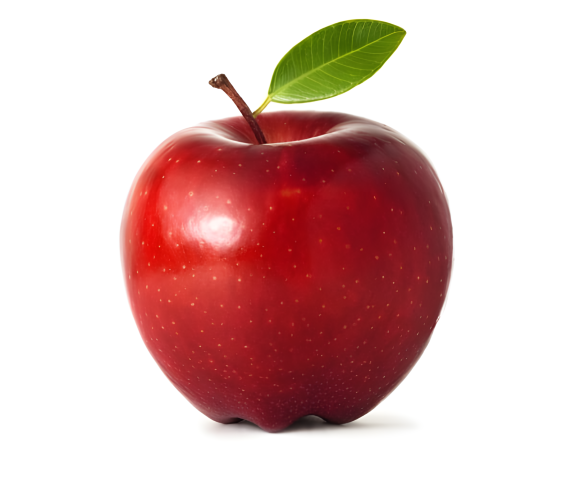
\includegraphics[width=\linewidth]{images/red-apple.png}
                          \captionof{figure}{\gcite{\href{https://www.bodi.com/blog/types-of-apples}{Source}}}
                          %
                          \column{0.1\linewidth}
                          \centering
                          $\xrightarrow{\rule{\linewidth}{0pt}}$
                          \column{0.45\linewidth}
                          This apple is red.
                      \end{columns}
                  \end{minipage}
              \end{center}
        \item \bhighlight{Logical atomism} is the view that reality consists of simple, independent facts (“atomic facts”) and that complex statements can be analyzed into combinations of these basic facts.
    \end{itemize}
\end{frame}

\begin{frame}{What is knowledge?}
    \begin{itemize}
        \item
              Is it the ability to predict interactions and events?
              \vspace{1em}
              \begin{center}
                  \begin{minipage}{0.7\textwidth}
                      \begin{columns}[c]
                          \column{0.45\linewidth}
                          \centering
                          Apples fall downward when dropped from a tree.
                          \column{0.1\linewidth}
                          \centering
                          $\xrightarrow{\rule{\linewidth}{0pt}}$
                          \column{0.45\linewidth}
                          \centering
                          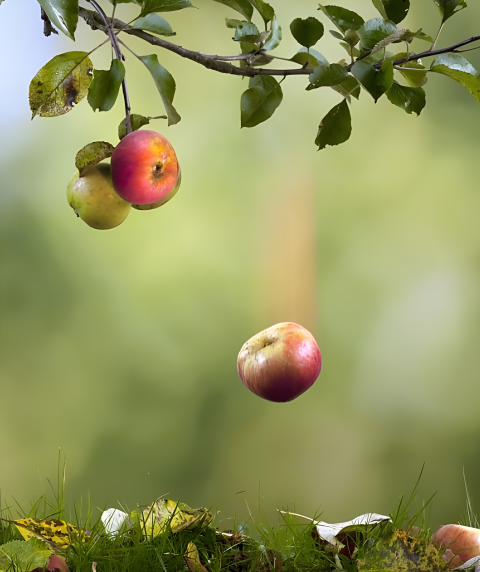
\includegraphics[width=\linewidth]{images/apple-falling.png}
                          \captionof{figure}{\gcite{\href{https://uk.pinterest.com/pin/prints-of-picture-no-10946968--794955771754853849/}{Source}}}
                      \end{columns}
                  \end{minipage}
              \end{center}
        \item \bhighlight{Instrumentalism} holds that the primary value of a theory or proposition is its \bhighlight{predictive} (and practical) efficacy—even if it doesn't claim to mirror some deeper reality.
    \end{itemize}
\end{frame}

\begin{frame}{What is knowledge?}
    \begin{itemize}
        \item
              Is ``verifiability'' important?
              \vspace{1em}
              \begin{center}
                  \begin{minipage}{0.7\textwidth}
                      \begin{columns}[c]
                          \column{0.45\linewidth}
                          Somewhere in the universe, there exists an apple that will ``fall'' upwards if no one is around to check.
                          \column{0.10\linewidth}
                          \centering
                          $\xleftrightarrow{\hspace*{0.5\linewidth}?\hspace*{0.5\linewidth}}$
                          \column{0.45\linewidth}
                          \centering
                          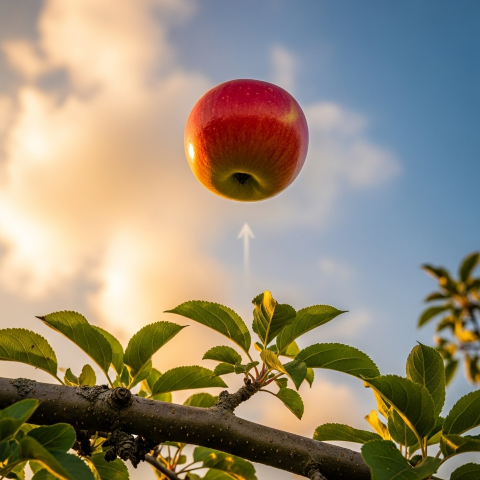
\includegraphics[width=\linewidth]{images/apple-rising.png}
                          \captionof{figure}{\gcite{\href{https://deepmind.google/models/imagen/}{Source}}}
                      \end{columns}
                  \end{minipage}
              \end{center}
        \item \bhighlight{Logical empiricism} expands on \bhighlight{logical atomism} to add a \bhighlight{verifiability} constraint. In order for a proposition to be meaningful,
              it needs to be verifiable, even if only in theory.
    \end{itemize}
\end{frame}
% \begin{frame}{Pragmatism}
    \begin{columns}[c]
        \column{0.8\columnwidth}
        \begin{itemize}
            \item Many views, we'll \emph{mostly} focus on one:
            \begin{cquote}
                Knowledge is any rule or practice that ``works''.
            \end{cquote}
            \item Basically, we'll consider some rule or pattern \bhighlight{true} if the predictions we make according to it turn out correct.
            \item Known as \bhighlight{Pragmatism}.
        \end{itemize}
        \column{0.2\columnwidth}
        \begin{figure}
                \centering
                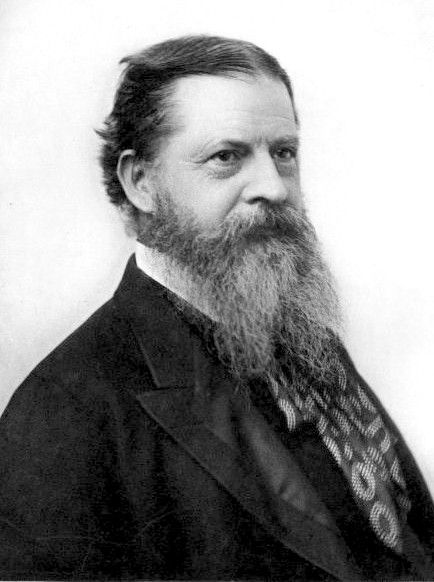
\includegraphics[width=\columnwidth]{images/Charles_Sanders_Peirce.jpg} % replace with your image file
                \caption{Charles Sanders Peirce --- mathematician and philosopher, and considered to be the father of Pragmatism. \gcite{\href{https://en.wikipedia.org/wiki/File:Charles_Sanders_Peirce.jpg}{Source}}}
            \end{figure}
    \end{columns}
\end{frame}

% \begin{frame}{Pragmatism}
%     \begin{columns}[c]
%         \begin{column}{0.80\textwidth}
%             \vfill
%             \begin{quote}
%                 ``All models are wrong, but some are useful." --- George Box
%             \end{quote}
%             \vfill
%         \end{column}
%         \begin{column}{0.20\textwidth}
%             \begin{figure}
%                 \centering
%                 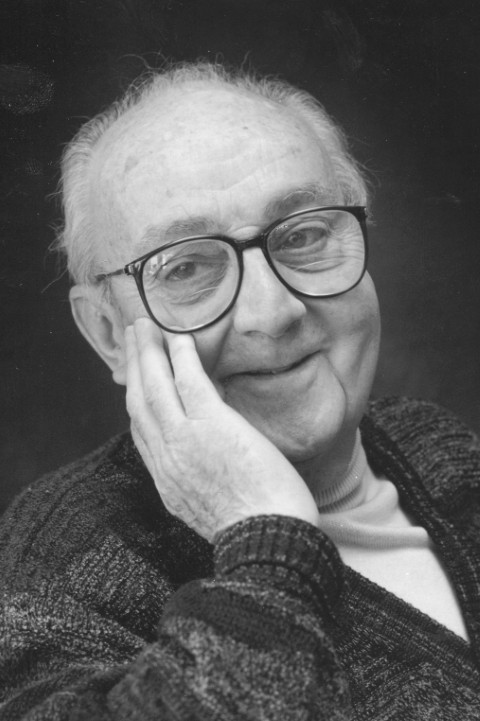
\includegraphics[width=\columnwidth]{images/george-ep-box.jpg} % replace with your image file
%                 \caption{George E.P. Box --- One of the great statistians of the 20th century. \gcite{\href{https://commons.wikimedia.org/w/index.php?curid=115167166}{Source}}}
%             \end{figure}
%         \end{column}
%     \end{columns}
% \end{frame}

% \begin{frame}{The pragmatic cycle}
%     \begin{figure}
%         \centering
%         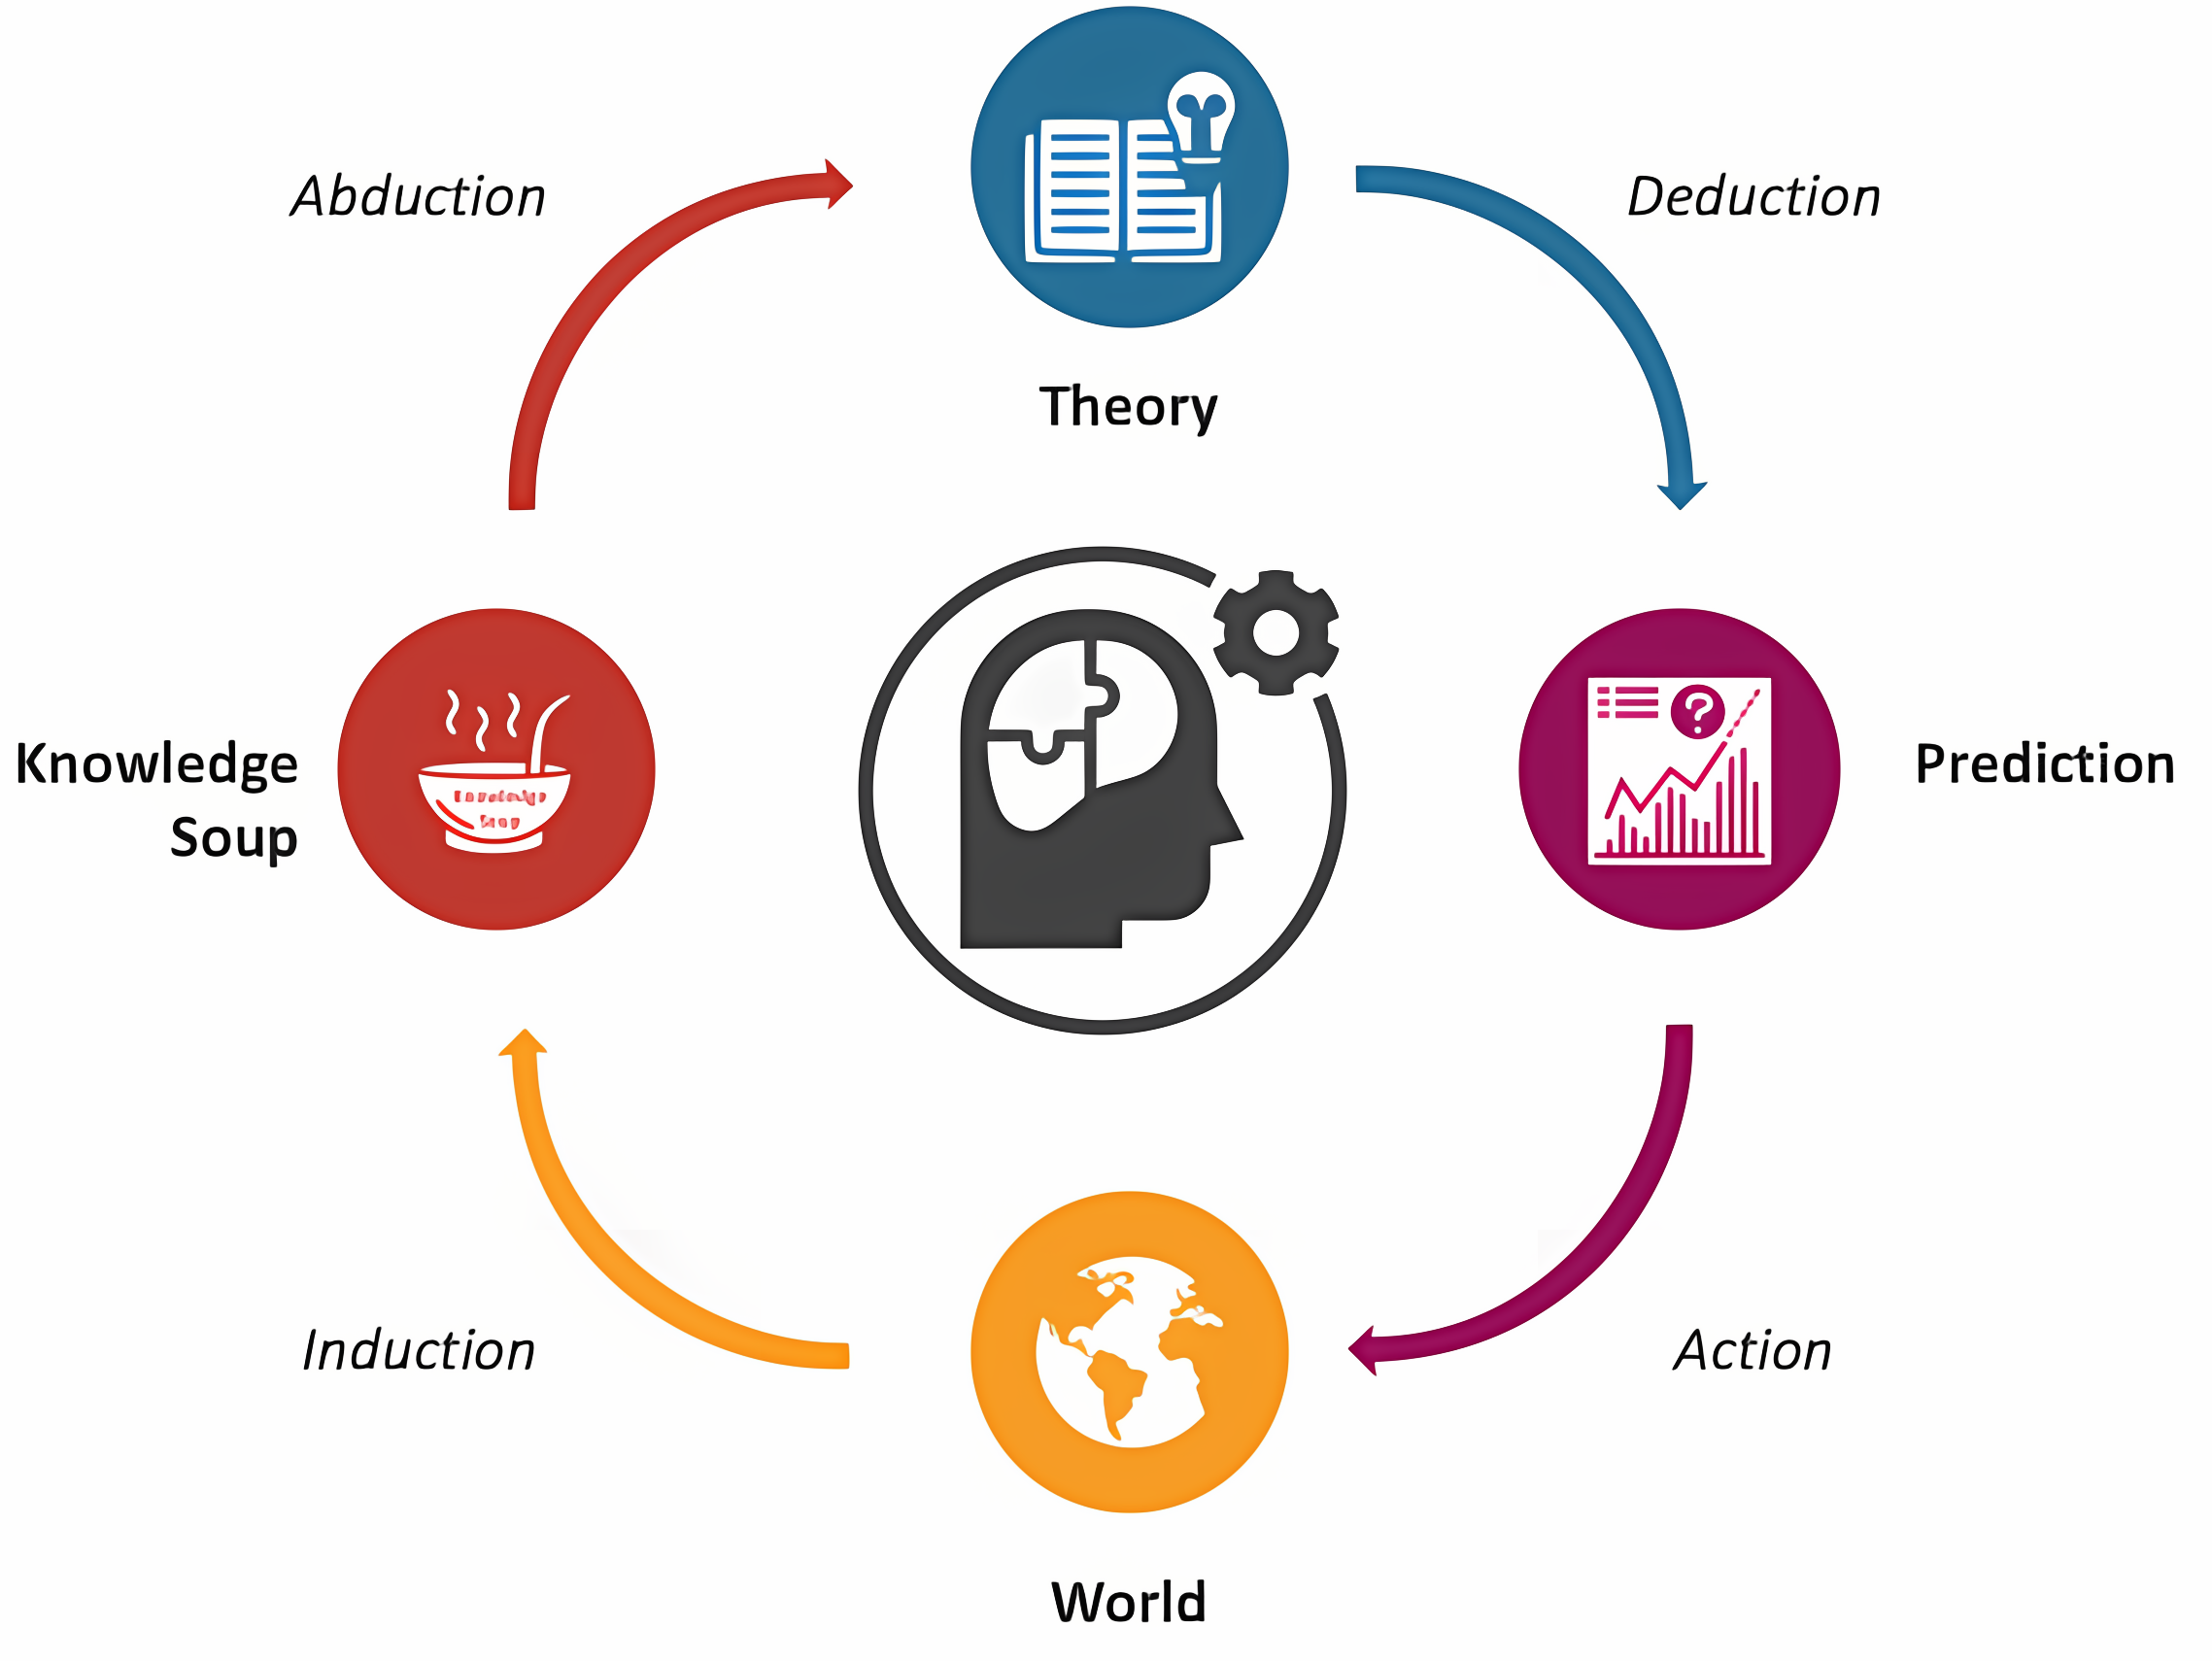
\includegraphics[width=0.8\textwidth]{images/pragmatism.png}
%         \caption{Peirce's cycle of Pragmatism. \gcite{\href{https://www.collidu.com/presentation-pragmatism}{Source}}}
%     \end{figure}
% \end{frame}
% \begin{frame}{Learning}
    \framesubtitle{Knowledge Acquisition}
    \begin{itemize}
        \item A natural follow-up question after categorizing knowledge is to ask: ``How do we, or any other \emph{intelligent} entity, obtain knowledge?''
        \item We call the process of knowledge-acquisiton \bhighlight{learning}.
        \item We'll discuss three beliefs that played critical roles in the formative years of AI, which will hopefully demystify the direction AI research has taken during the last few decades.
    \end{itemize}
\end{frame}

% Symbolism
\begin{frame}{Symbolism}
    \framesubtitle{The Symbolic Paradigm}
    \begin{itemize}
        \item The core idea within \bhighlight{symbolism} is that knowledge lives in discrete chunks called \bhighlight{symbols} and the mind is a ``symbol processing machine''. \\
        \item Symbolists posit the existence of a mental \bhighlight{language} akin to natural human language, where thoughts are formed via \bhighlight{logical} ($\land$, $\lor$, $\neg$, $\implies$) combinations
              of the \emph{words} within this language.
        \item In this view, the mind is much like a machine processing a list of instructions.
    \end{itemize}
\end{frame}

\begin{frame}{Symbolism}
    \framesubtitle{Symbolic Reasoning Diagram}
    \begin{figure}
        \centering
        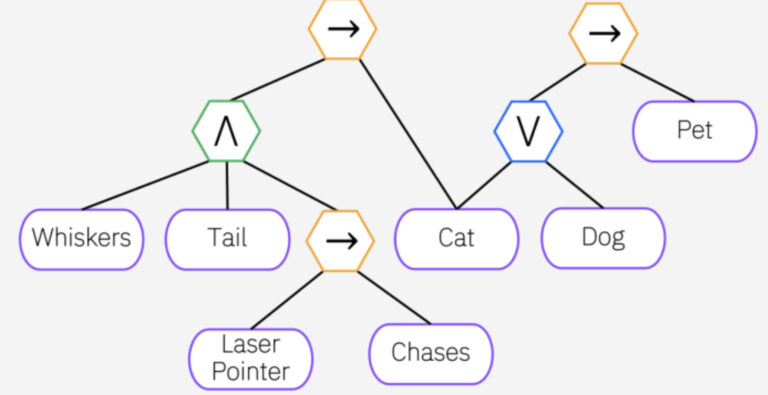
\includegraphics[width=0.8\linewidth]{images/symbolic-ai.jpg}
        \caption{A simplified logical decomposition of a thought. \gcite{\href{https://startupkitchen.community/neuro-symbolic-ai-why-is-it-the-future-of-artificial-intelligence/}{Source}}}
    \end{figure}
\end{frame}

\begin{frame}{Symbolism}
    \framesubtitle{History}
    \begin{itemize}
        \item This view dominated the field of AI between the mid-1950s and the mid-1990s.
        \item Classical AI such as \bhighlight{decision trees} or \bhighlight{rule-based systems} followed this philosophy.
        \item Such systems are now dubbed \bhighlight{GOFAI} (good old-fashioned artificial intelligence).
        \item A key feature of these systems was their \bhighlight{transparent} decision making, a feature somewhat lost in modern approaches such as neural networks,
              which has led to a resurgence of symbolic AI in hybrid approaches called \bhighlight{neuro-symbolic} AI.
    \end{itemize}
\end{frame}

% Associationism
\begin{frame}{Associationism}
    \framesubtitle{Linking Ideas through Experience}
    \begin{itemize}
        \item Historically preceding symbolism yet paramount to subsequent theories of intelligence, \bhighlight{associationism} states that minds form knowledge by linking ideas through experience.
        \item One of the most foundational works in explaining how neurons learn is the theory of \bhighlight{Hebbian learning}, which applies the associative principle of learning to the brain:
              ``neurons that fire together wire together.''
    \end{itemize}
\end{frame}

\begin{frame}{Associationism}
    \framesubtitle{Principles of Associative Learning}
    The classical ``laws'' of association are as follows:
    \begin{itemize}
        \item \textbf{Contiguity:} Things that occur together in time or space become linked (e.g., lightning and thunder).
        \item \textbf{Similarity:} Things that share features become linked (e.g., thinking of an apple might make you think of a pear).
        \item \textbf{Contrast:} Opposites become linked (e.g., thinking of hot brings up cold).
        \item \textbf{Repetition:} Things paired often become strongly linked (e.g., hearing a song every morning ties it to waking up).
    \end{itemize}
\end{frame}

\begin{frame}{Associationism}
    \framesubtitle{Pavlov’s Conditioning}
    A famous example of associative learning is \bhighlight{Pavlov's dog} experiment, which explores classical conditioning:
    \begin{figure}
        \centering
        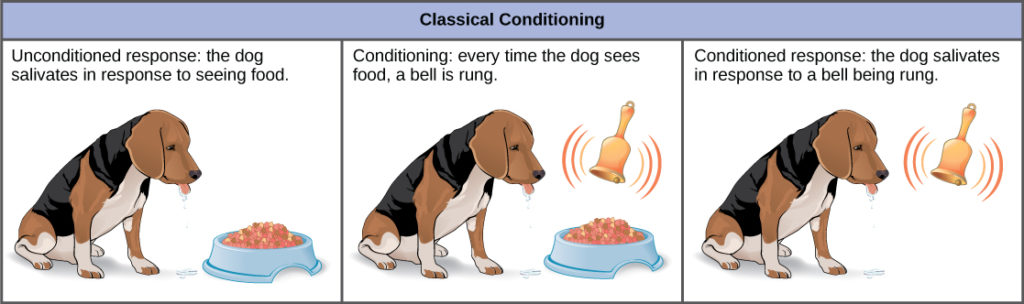
\includegraphics[width=\linewidth]{images/pavlov-dog.jpg}
        \caption{Pavlov's experiment. \gcite{\href{https://courses.lumenlearning.com/wm-biology2/chapter/learned-behaviors/}{Source}}}
    \end{figure}
\end{frame}

% Connectionism
\begin{frame}{Connectionism}
    \framesubtitle{Distributed Representations}
    \begin{itemize}
        \item \bhighlight{Connectionism} posits that knowledge arises from networks of interconnected, simple processing units inspired by neural structures in biological brains.
        \item Unlike symbolism, connectionism does not rely on explicit symbolic representations but rather on distributed representations across many units (neurons).
        \item Knowledge is represented implicitly in the \bhighlight{connections} between units and the \bhighlight{strengths (weights)} of these connections.
    \end{itemize}
\end{frame}

\begin{frame}{Connectionism}
    \framesubtitle{Training Connectionist Networks}
    \begin{itemize}
        \item Connectionism emphasizes \bhighlight{parallel distributed processing (PDP)}—many interconnected processing elements working simultaneously.
        \item Learning in connectionism occurs by adjusting the connection strengths (weights) based on experience, a process called \bhighlight{training}.
        \item Connectionist training often uses \bhighlight{gradient-based learning}, where weights are nudged little by little in the direction that reduces error, and an \bhighlight{expectation–maximization (EM)} style approach, which alternates between guessing how each part of the network contributes to the task and then updating the weights to improve performance.
    \end{itemize}
\end{frame}

\begin{frame}{Connectionism}
    \framesubtitle{Structure of an Artificial Neural Network}
    \begin{figure}
        \centering
        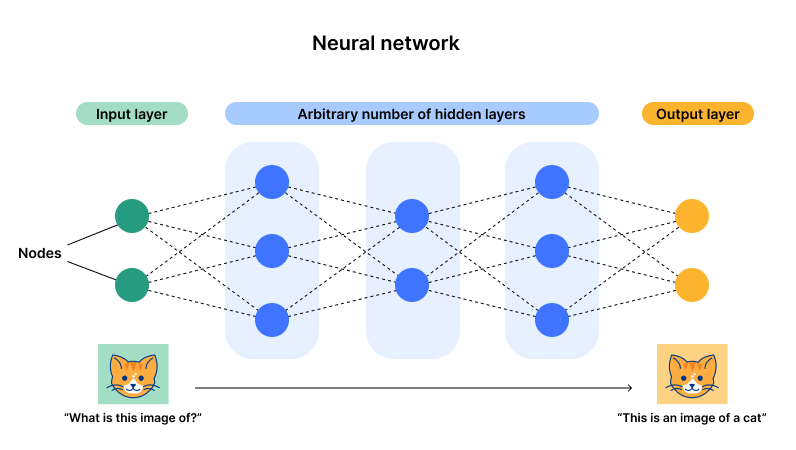
\includegraphics[width=\linewidth]{images/neural-network.png}
        \caption{An artificial neural network (ANN) composed of interconnected nodes, inspired by biological neural networks. \gcite{\href{https://www.cloudflare.com/learning/ai/what-is-neural-network/}{Source}}}
    \end{figure}
\end{frame}

\begin{frame}{Connectionism}
    \framesubtitle{Rise of Deep Learning}
    \begin{columns}[c]
        \begin{column}{0.6\linewidth}
            \begin{itemize}
                \item Connectionism rose to prominence in the 1980s and is the foundation for modern \bhighlight{deep learning}, the dominant approach in AI today.
                \item Models like \bhighlight{artificial neural networks} excel at pattern recognition and learning but their lack of interpretability drives ongoing research in explainable AI.
            \end{itemize}
        \end{column}
        %
        \begin{column}{0.4\linewidth}
            \begin{figure}
                \centering
                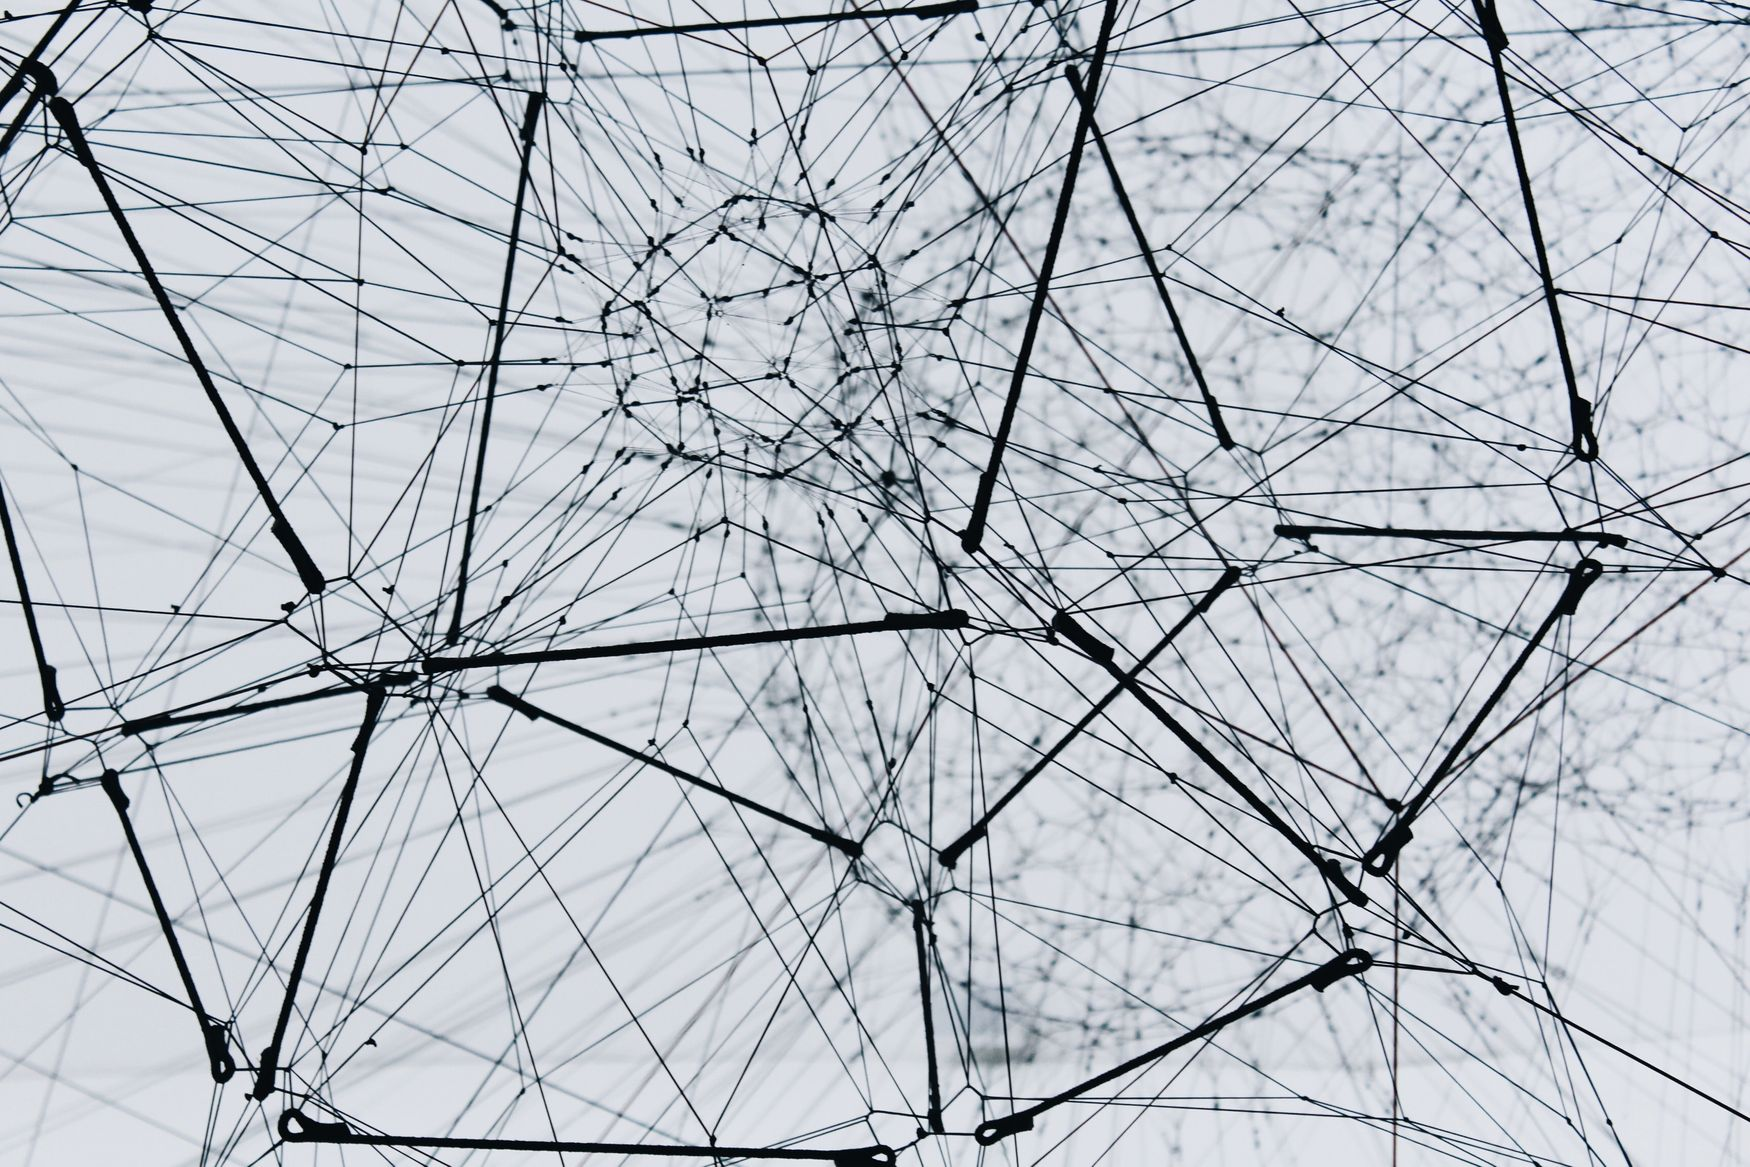
\includegraphics[width=\columnwidth]{images/connectionism.jpg}
                \caption{Photo of an interconnected metal structure, resembling connectionist machines. \gcite{\href{https://unsplash.com/photos/low-angle-photography-of-metal-structure-ZiQkhI7417A}{Source}}}
            \end{figure}
        \end{column}
    \end{columns}
\end{frame}
% \begin{frame}{Models as Approximations}
  \begin{columns}[c]
    \begin{column}{0.8\linewidth}
      \begin{itemize}
        \item Human minds and artificial systems never grasp reality directly; we use simplified representations called \bhighlight{models}.
        \item George E.P. Box famously stated: \\
              \emph{``All models are wrong, but some are useful.''}
        \item Our goal isn't perfect truth, but \bhighlight{useful approximations} that help us predict and interact with the world.
      \end{itemize}
    \end{column}
    \begin{column}{0.2\linewidth}
      \begin{figure}
        \centering
        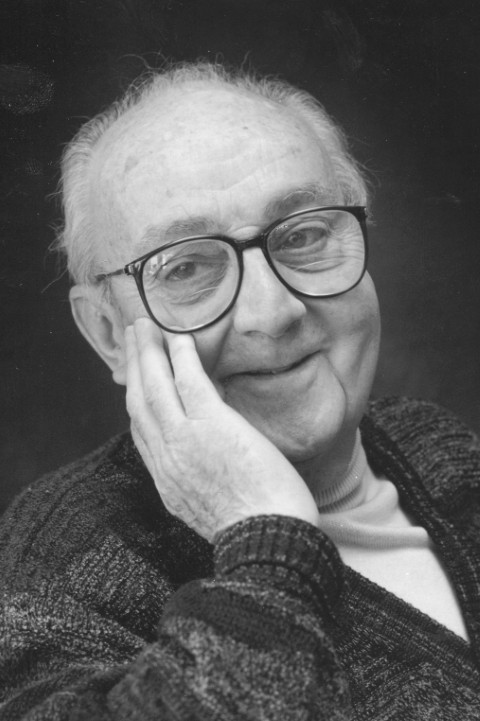
\includegraphics[width=\columnwidth]{images/george-ep-box.jpg}
        \caption{George E.P. Box --- One of the great statistians of the 20th century. \gcite{\href{https://commons.wikimedia.org/w/index.php?curid=115167166}{Source}}}
      \end{figure}
    \end{column}
  \end{columns}
\end{frame}

\begin{frame}{Observations and Reality}
  \begin{columns}[c]
    \begin{column}{0.6\linewidth}
      \begin{itemize}
        \item Our understanding comes from \bhighlight{observations}, which are samples or instances of reality.
        \item We assume there's an underlying \bhighlight{data-generating process} that creates the data we observe.
      \end{itemize}
    \end{column}
    %
    \begin{column}{0.4\linewidth}
      \begin{figure}
        \centering
        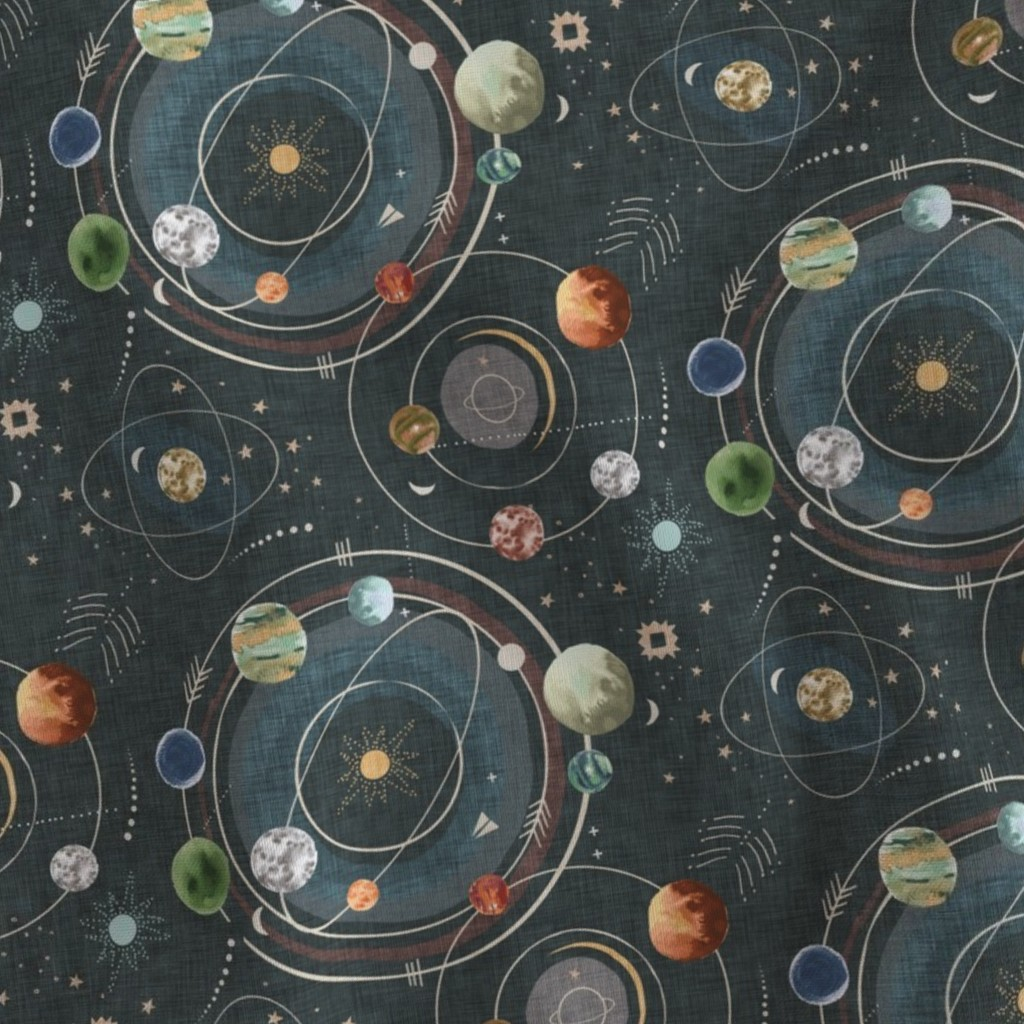
\includegraphics[width=\columnwidth]{images/universe.jpg}
        \caption{The data-generating process in our universe is the hidden ``source code'' that makes the laws of physics be the way they are. \gcite{\href{https://www.spoonflower.com/en/fabric/11122531-space-map-charcoal-med-by-nouveau_bohemian}{Source}}}
      \end{figure}
    \end{column}
  \end{columns}
\end{frame}

\begin{frame}{Observations and Reality}
  \begin{itemize}
    \item If our observations are good representations, we can learn rules and patterns that \bhighlight{generalize} to new situations.
    \item But how do we choose between multiple possible models?
  \end{itemize}
\end{frame}

\begin{frame}{Maximum Likelihood}
  \framesubtitle{Choosing the Best Model}
  \begin{itemize}
    \item A widely-used principle for selecting a model is \bhighlight{maximum likelihood}.
    \item Intuitively, it means choosing the model under which the observed data would have the \emph{highest probability} of occurring.
    \item Imagine flipping a coin:
          \begin{itemize}
            \item If you see heads 90 out of 100 times, which is more likely—a fair coin, or a biased one?
          \end{itemize}
    \item Maximum likelihood helps us quantify this intuition mathematically, guiding our choice of models based on observations.
  \end{itemize}
\end{frame}

% -------------------------------------------------------------------
\begin{frame}{Model Parameters}
  \framesubtitle{Defining a Hypothesis Space}
  \begin{itemize}
    \item A \bhighlight{model} is really a family of possible explanations for our data.
    \item We index each candidate by a vector of \bhighlight{parameters} $\theta\in\Theta$:
          \[
            p(x \mid \theta), \quad \theta = (\theta_1, \theta_2, \dots).
          \]
    \item Changing $\theta$ “moves” us to a different hypothesis about how data were generated.
    \item Learning = selecting the best $\theta$ given what we've actually observed.
  \end{itemize}
\end{frame}

\begin{frame}{Model Parameters}
  % \framesubtitle{...}
  \begin{figure}
    \centering
    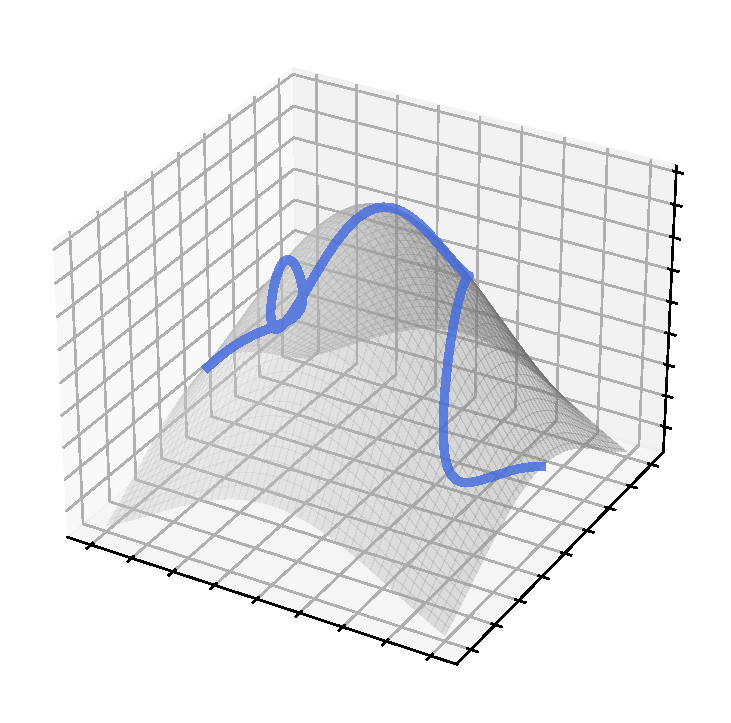
\includegraphics[height=0.65\textheight]{images/model_family_on_hypothesis_space.pdf}
    \caption{Visualization of a model family (red 2D curve) over a hypothesis space (transparent 3D curve).}
  \end{figure}
\end{frame}

% -------------------------------------------------------------------
\begin{frame}{The Likelihood Function}
  \framesubtitle{How Well Does $\theta$ Explain the Data?}
  \begin{itemize}
    \item Suppose our dataset is $D = \{x_1, x_2, \dots, x_N\}$.
    \item We quantify the \emph{fit} of parameters $\theta$ via the \bhighlight{likelihood}:
          \[
            L(\theta;D) \;=\;\prod_{i=1}^N p\bigl(x_i \mid \theta\bigr).
          \]
    \item Rather than “probability of $\theta$,” think of $L(\theta;D)$ as “how plausible is $\theta$ \emph{given} the observed data?”
    \item Larger $L(\theta)$ means the model under $\theta$ would have made our observations more likely.
  \end{itemize}
\end{frame}

\begin{frame}{The Likelihood Function}
  % \framesubtitle{...}
  \begin{figure}
    \centering
    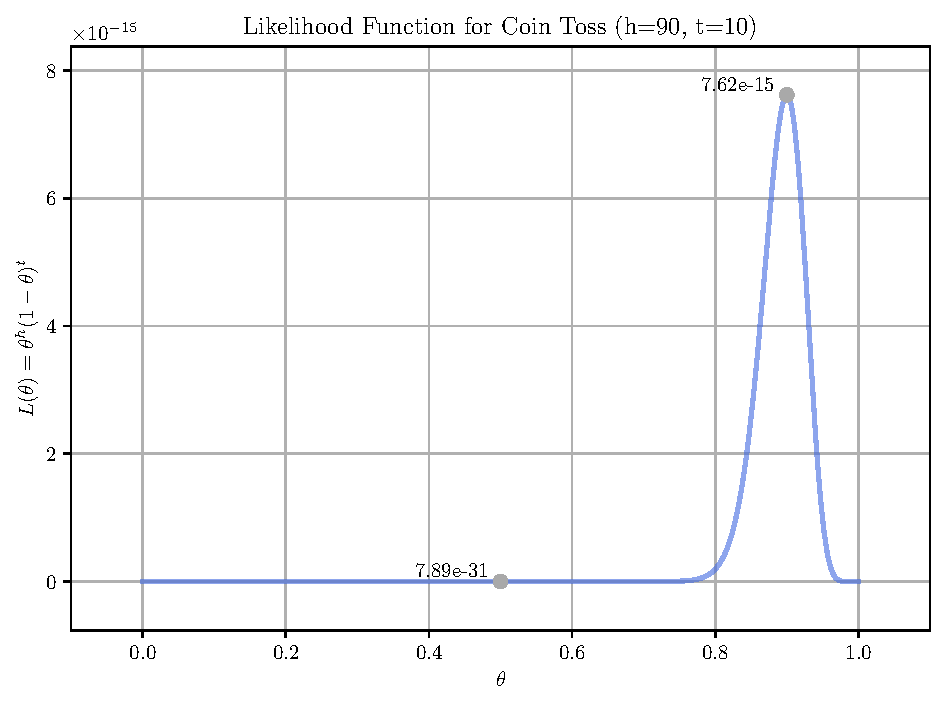
\includegraphics[height=0.65\textheight]{images/coin_toss_likelihood.pdf}
    \caption{Likelihood plot for a biased coin.}
  \end{figure}
\end{frame}

% -------------------------------------------------------------------
\begin{frame}{Log-Likelihood}
  \framesubtitle{Simplifying Optimization}
  \begin{itemize}
    \item Products can get unwieldy; take logs to turn products into sums:
          \[
            \ell(\theta;D) \;=\;\log L(\theta;D)
            \;=\;\sum_{i=1}^N \log p(x_i \mid \theta).
          \]
    \item $\ell(\theta)$ is called the \bhighlight{log-likelihood}.
    \item Maximizing $\ell(\theta)$ is equivalent to maximizing $L(\theta)$, but often easier to differentiate.
    \item In many cases we find a closed-form solution; otherwise we use \bhighlight{gradient-based} search which will be explored in later lectures.
  \end{itemize}
\end{frame}

\begin{frame}{Log-Likelihood}
  % \framesubtitle{...}
  \begin{figure}
    \centering
    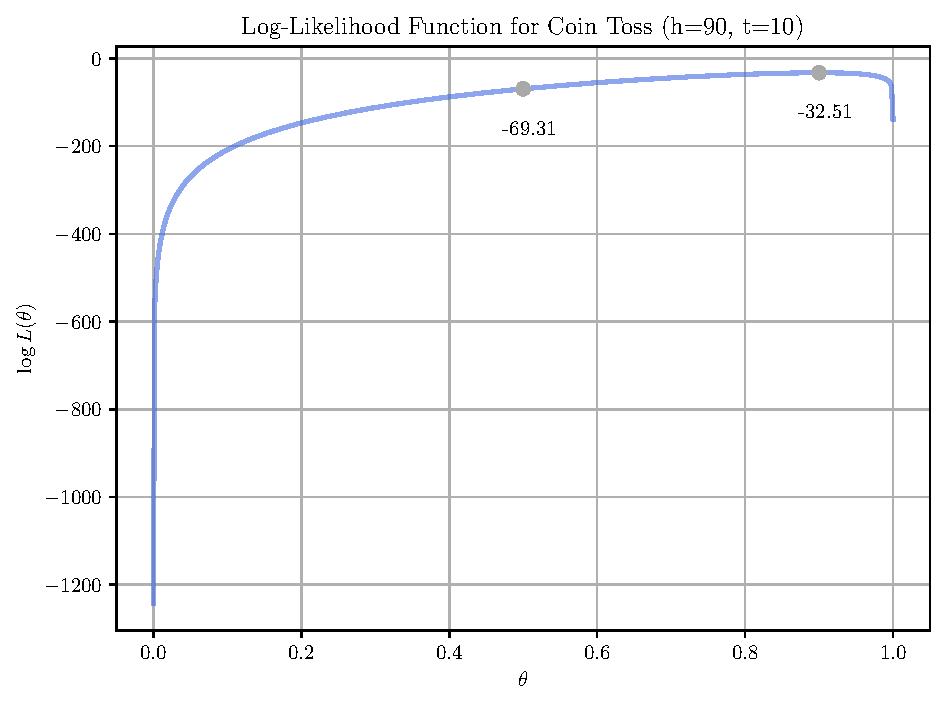
\includegraphics[height=0.65\textheight]{images/coin_toss_log_likelihood.pdf}
    \caption{Log-likelihood plot for the same biased coin as before.}
  \end{figure}
\end{frame}

% -------------------------------------------------------------------
\begin{frame}{Maximum Likelihood Estimation}
  \framesubtitle{Picking the Best Parameters}
  \begin{itemize}
    \item The core rule is
          \[
            \hat\theta_{\text{MLE}}
            \;=\;
            \argmax_{\theta\in\Theta}\;L(\theta;D)
            \;=\;
            \argmax_{\theta}\;\ell(\theta;D).
          \]
    \item This is our formal definition of “learning” in a statistical model:
          choose the hypothesis (parameters) under which the data are most probable.
  \end{itemize}
\end{frame}

% -------------------------------------------------------------------
{
\setframecolor{Crimson}
\begin{frame}{Coin Toss Pop Quiz}
  \framesubtitle{Estimating a Biased Coin}
  \begin{itemize}
    \item Each trial \(x_i\) is either heads (\(\mathrm{H}\)) or tails (\(\mathrm{T}\)); our model assumes \(\theta\) is the probability of heads.
    \item \textbf{Q1:} Write down the likelihood \(L(\theta)\) for observing \(h\) heads and \(t\) tails.
    \item \textbf{Q2:} Express the log-likelihood \(\ell(\theta)\).
    \item \textbf{Q3:} Compute the value of \(\theta\) that maximizes \(\ell(\theta)\).
  \end{itemize}
\end{frame}

\begin{frame}{Coin Toss Example — Solutions}
  \framesubtitle{Estimating a Biased Coin}
  \begin{itemize}
    \item \textbf{Likelihood:}
          \[
            L(\theta)
            = \theta^{\,h}\,(1-\theta)^{\,t}.
          \]
    \item \textbf{Log-likelihood:}
          \[
            \ell(\theta)
            = h\log\theta \;+\; t\log(1-\theta).
          \]
    \item \textbf{Maximizer:}
          \[
            \frac{d\ell}{d\theta}
            = \frac{h}{\theta} - \frac{t}{1-\theta} = 0
            \;\Longrightarrow\;
            \hat\theta = \frac{h}{h+t}.
          \]
    \item \emph{Intuition: “frequency = probability.”}
  \end{itemize}
\end{frame}
}

% -------------------------------------------------------------------
\begin{frame}{What Is a Random Variable?}
  \framesubtitle{From Real-World to Numbers}
  \begin{itemize}
    \item A \bhighlight{random variable} $X$ is just a way to turn an uncertain outcome into a number.
    \item Examples:
          \begin{itemize}
            \item Tossing a coin: $X=1$ for heads, $0$ for tails.
            \item Measuring temperature: $X$ = today's temperature in °C.
          \end{itemize}
    \item Each possible outcome has some \emph{chance} (probability) of happening.
  \end{itemize}
\end{frame}

% -------------------------------------------------------------------
\begin{frame}{The ``True'' Average (Expectation)}
  \framesubtitle{What We'd Get with Infinite Data}
  \begin{itemize}
    \item If we could repeat an experiment forever, the \bhighlight{expected value} (or \emph{population mean}) of $X$ is:
          \[
            \mu = \mathbb{E}[X] \;=\; \sum_x x\cdot P(X=x)
            \quad\bigl(\text{or } \int x\,p(x)\,dx\bigr).
          \]
    \item Informally: “where would the average settle if we could sample forever?”
    \item In practice, we don't know $\mu$ because we can't sample infinitely.
  \end{itemize}
\end{frame}

% -------------------------------------------------------------------
\begin{frame}{Sample Mean}
  \framesubtitle{What We Actually Observe}
  \begin{itemize}
    \item Suppose we collect $N$ measurements: $X_1, X_2, \dots, X_N$.
    \item Their \bhighlight{sample mean} is
          \[
            \overline{X} = \frac{1}{N}\sum_{i=1}^N X_i.
          \]
    \item This is the average we compute on our finite data.
    \item Question: \emph{How close} is $\overline{X}$ to the true mean $\mu$?
  \end{itemize}
\end{frame}

% -------------------------------------------------------------------
\begin{frame}{Law of Large Numbers}
  \framesubtitle{How ``quantity'' can improve ``quality''}
  \begin{itemize}
    \item The \bhighlight{Law of Large Numbers} says:
          \[
            \bar X \;\to\; \mu
            \quad\text{as}\quad N\to\infty.
          \]
    \item In plain terms: “With more data, the sample mean gets closer to the true mean.”
    \item This justifies using $\overline{X}$ as an estimate for $\mu$ when $N$ is large.
  \end{itemize}
\end{frame}

\begin{frame}{Law of Large Numbers}
  % \framesubtitle{...}
  \begin{figure}
    \centering
    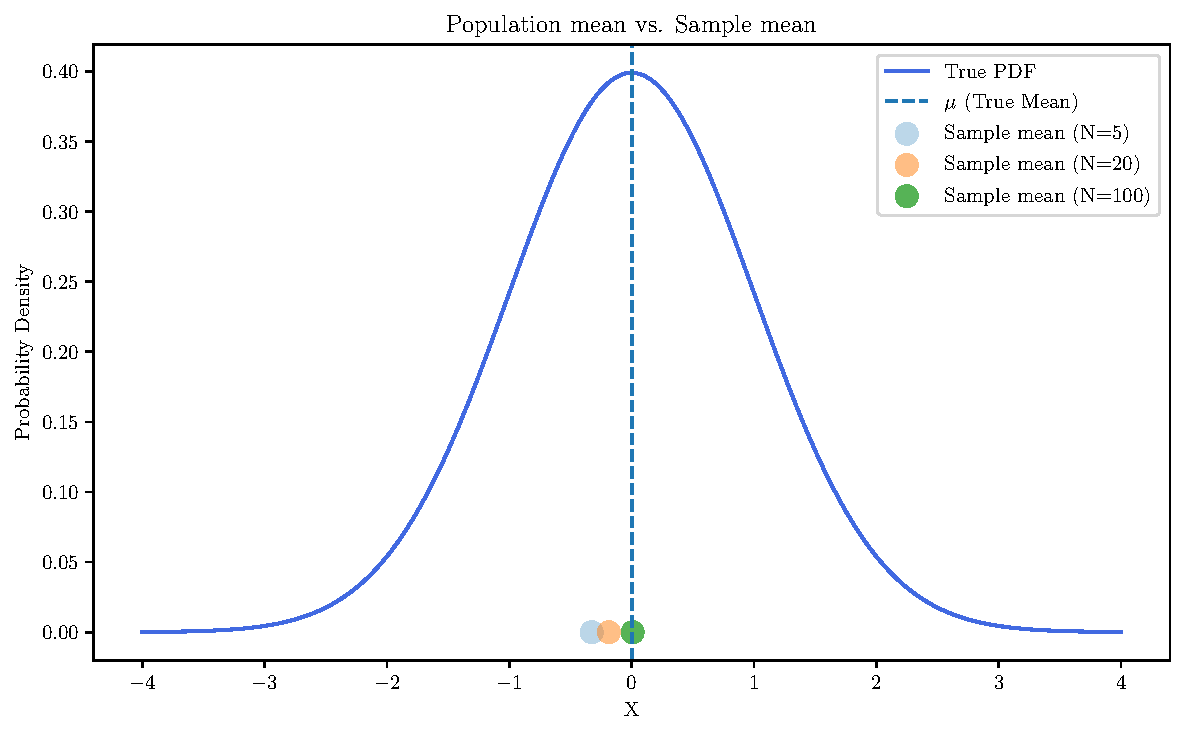
\includegraphics[height=0.65\textheight]{images/pop_mean_vs_sample_mean.pdf}
    \caption{Sample mean for three samples of the Normal distribution.}
  \end{figure}
\end{frame}

% -------------------------------------------------------------------
\begin{frame}{Measuring our mistakes}
  \framesubtitle{Loss functions}
  \begin{itemize}
    \item In learning we make predictions $f(x;\theta)$ and compare to true $y$.
    \item A \bhighlight{loss function} $\ell(y, f(x;\theta))$ assigns a \emph{numeric cost} to each mistake.
    \item Examples:
          \[
            \ell_{\text{0-1}} = \begin{cases}0 & \text{correct}\\1 & \text{wrong}\end{cases}
            ,\quad
            \ell_{\text{sq}}=(y - f(x))^2.
          \]
  \end{itemize}
\end{frame}

% -------------------------------------------------------------------
\begin{frame}{True Risk vs.\ Empirical Risk}
  \framesubtitle{Infinite Data vs.\ Finite Data}
  \begin{itemize}
    \item \bhighlight{True risk}:
          \[
            R(\theta)
            = \mathbb{E}\bigl[\ell(y, f(x;\theta))\bigr]
            \quad\text{(if we had infinite data).}
          \]
    \item \bhighlight{Empirical risk} (what we compute):
          \[
            \hat R(\theta)
            = \frac{1}{N}\sum_{i=1}^N \ell\bigl(y_i, f(x_i;\theta)\bigr).
          \]
    \item By the Law of Large Numbers, $\hat R(\theta)\approx R(\theta)$ when $N$ is large.
  \end{itemize}
\end{frame}

% -------------------------------------------------------------------
\begin{frame}{Empirical Risk Minimization}
  \framesubtitle{Learning as “Minimize Your Mistakes”}
  \begin{itemize}
    \item Since we can’t see $R(\theta)$, we pick
          \[
            \hat\theta
            = \argmin_{\theta}\;\hat R(\theta)
            = \argmin_{\theta}\;\frac{1}{N}\sum_{i=1}^N \ell(y_i, f(x_i;\theta)).
          \]
    \item Intuitively: “find the parameters that make your average mistake as small as possible.”
    \item This simple rule underlies nearly all supervised learning methods!
  \end{itemize}
\end{frame}
% -------------------------------------------------------------------

% End

\begin{frame}{The Goal: A Functional View}
    \framesubtitle{What are we trying to build?}
    \small
    \begin{itemize}
        \item At a high level, many tasks in AI can be seen as learning a complex \bhighlight{function} that maps a given input to a desired output.
        \item A neural network is a powerful tool for modeling such functions. Our goal is to find the right network that performs the specific mapping we need.
    \end{itemize}
    \begin{figure}
        \centering
        % Source: MLP & Back-prop.pdf, Page: 2
        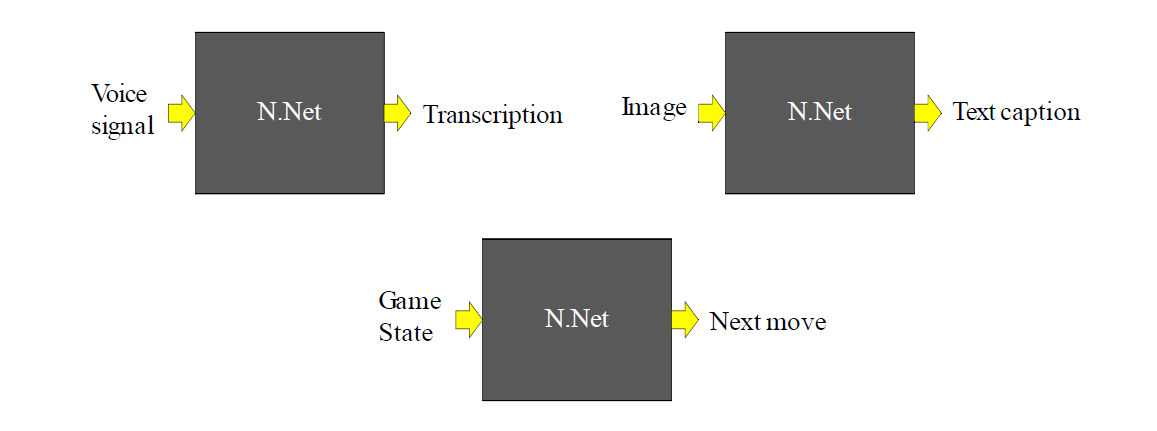
\includegraphics[width=0.9\linewidth]{images/nn_as_function.png}
        \caption{Neural networks act as functions mapping inputs (like voice or images) to outputs (like text or actions).}
    \end{figure}
\end{frame}

\begin{frame}{The Goal: The Formal Problem Setup}
    \framesubtitle{What we have and what we want}
    Based on the previous slides, we can formally define our task:
    \begin{itemize}
        \item \textbf{Given:}
        \begin{itemize}
            \item The \bhighlight{architecture} of the network (e.g., number of layers and neurons).
            \item A set of N \bhighlight{training data} pairs: $(x^{(1)}, y^{(1)}), (x^{(2)}, y^{(2)}), \dots, (x^{(N)}, y^{(N)})$.
        \end{itemize}
        \medskip
        \item \textbf{To Find:}
        \begin{itemize}
            \item The optimal set of \bhighlight{parameters} (weights and biases, denoted collectively as $W$) for our network.
        \end{itemize}
    \end{itemize}
\end{frame}

% --- SLIDE WITH CORRECTION ---
\begin{frame}{The Goal: The Parametric Function and Cost} 
    \framesubtitle{Representing the Network and its Error}
    \begin{itemize}
        \item We consider a neural network as a \bhighlight{parametric function}, $f(x; W)$, where $W$ represents all learnable parameters.
        \item A \bhighlight{loss function}, $\text{loss}(f(x;W), y)$, penalizes the difference between the network's prediction and the desired output for a \emph{single} training example.
        \item The overall \bhighlight{Cost Function} $E(W)$ is the average loss over the \emph{entire} dataset:
        \[
            E(W) = \frac{1}{N} \sum_{n=1}^{N} \text{loss}(f(x^{(n)}; W), y^{(n)})
        \]
    \end{itemize}
\end{frame}

\begin{frame}{The Goal: A Key Requirement}
    \framesubtitle{The Need for Differentiability}
    \begin{itemize}
        \item Our goal is to minimize the cost $E(W)$. To do this with gradient-based methods, the cost function must be \bhighlight{differentiable} with respect to the weights $W$.
        \item This means we must use:
        \begin{itemize}
            \item \textbf{Differentiable Loss Functions:} The way we measure error must be smooth.
            \item \textbf{Continuous Activation Functions:} The functions inside our neurons (like Sigmoid or ReLU) must be differentiable, allowing gradients to flow through the network.
        \end{itemize}
    \end{itemize}
\end{frame}

\begin{frame}{Case Study: Regression}
    \framesubtitle{Output and Loss for Real-Valued Targets}
    \begin{itemize}
        \item For tasks where the desired output is a real number or a vector of real numbers (e.g., predicting a price).
        \item \textbf{Output Layer:} Typically has linear neurons (i.e., no activation function is applied).
        \item \textbf{Loss Function:} The most common choice is the \bhighlight{Squared Error} (or L2 loss):
        \[
            \text{loss}(y, o) = \frac{1}{2} \|y - o\|^2 = \frac{1}{2} \sum_k (y_k - o_k)^2
        \]
    \end{itemize}
    \begin{figure}
        \centering
        % Source: MLP & Back-prop.pdf, Page: 7
        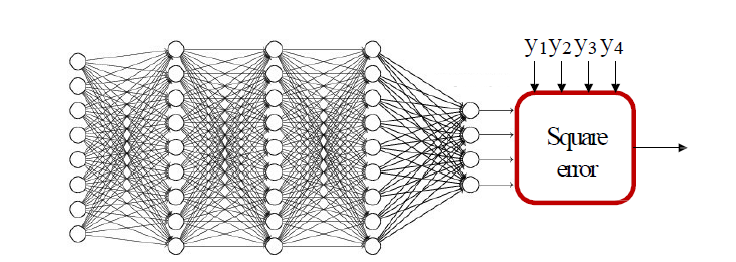
\includegraphics[width=0.8\linewidth]{images/loss_regression.png}
    \end{figure}
\end{frame}

\begin{frame}{Case Study: Binary Classification}
    \framesubtitle{Output and Loss for Two-Class Problems}
    \begin{itemize}
        \item For tasks with two classes (e.g., Cat vs. Dog), where the target $y$ is either 0 or 1.
        \item \textbf{Output Layer:} A single neuron with a \bhighlight{Sigmoid} activation function. This squashes the output to a range of (0, 1), which we can interpret as a probability $P(Y=1|x)$.
        \item \textbf{Loss Function:} \bhighlight{Binary Cross-Entropy} is the standard choice:
        \[
            \text{loss}(y, o) = -y \log(o) - (1 - y) \log(1 - o)
        \]
    \end{itemize}
    \begin{figure}
        \centering
        % Source: MLP & Back-prop.pdf, Page: 11
        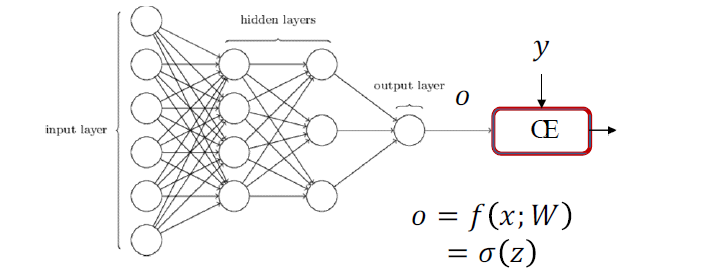
\includegraphics[width=0.6\linewidth]{images/loss_binary_ce.png}
    \end{figure}
\end{frame}

\begin{frame}{Case Study: Multi-Class Classification}
    \framesubtitle{Setup for K > 2 Classes}
    \begin{itemize}
        \item For tasks with multiple classes (e.g., MNIST digits 0-9).
        \item \textbf{Target Representation:} The desired output $y$ is represented as a \bhighlight{one-hot vector}. For example, for class 3 out of 5, $y = [0, 0, 1, 0, 0]^T$.
        \item \textbf{Output Layer:} Must have K neurons, one for each class.
        \item To ensure the outputs are probabilities that sum to 1, we need a special activation function.
    \end{itemize}
\end{frame}

\begin{frame}{Case Study: Multi-Class Classification}
    \framesubtitle{The Softmax Activation}
    \begin{itemize}
        \item The \bhighlight{Softmax} function is used as the activation for the output layer in multi-class problems.
        \item It takes a vector of raw scores (logits) $z$ and transforms it into a probability distribution $o$:
        \[
            o_i = \text{softmax}(z)_i = \frac{\exp(z_i)}{\sum_{j=1}^{K} \exp(z_j)}
        \]
        \item Each output $o_i$ is between 0 and 1, and all outputs sum to 1, making them valid probabilities.
    \end{itemize}
    \begin{figure}
        \centering
        % Source: MLP & Back-prop.pdf, Page: 13
        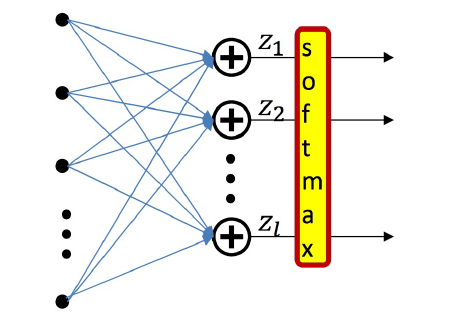
\includegraphics[width=0.5\linewidth]{images/softmax_layer.png}
        \caption{The softmax activation is applied to the final layer.}
    \end{figure}
\end{frame}

\begin{frame}{Case Study: Multi-Class Classification}
    \framesubtitle{Cross-Entropy Loss}
    \begin{itemize}
        \item \textbf{Loss Function:} For multi-class classification, we use the \bhighlight{Cross-Entropy} loss.
        \[
            \text{loss}(y, o) = -\sum_{i=1}^{K} y_i \log(o_i)
        \]
        \item Since $y$ is a one-hot vector, only one term in the sum is non-zero. If the true class is $c$, the formula simplifies to:
        \[
            \text{loss}(y, o) = - \log(o_c)
        \]
        \item This means we are trying to maximize the log-probability of the correct class.
    \end{itemize}
    \begin{figure}
        \centering
        % Source: MLP & Back-prop.pdf, Page: 15
        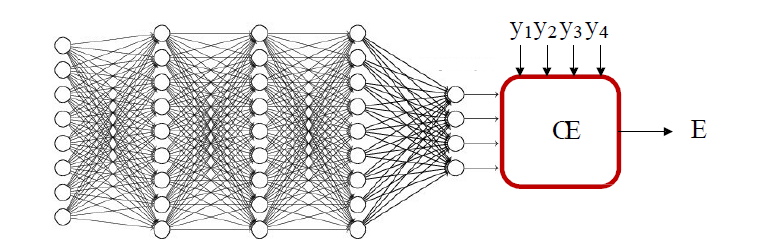
\includegraphics[width=0.8\linewidth]{images/loss_multiclass_ce.png}
    \end{figure}
\end{frame}

\begin{frame}{The Tool: Gradient Descent}
    \framesubtitle{The Core Idea}
    \begin{itemize}
        \item We use an iterative optimization algorithm called \bhighlight{gradient descent} to find the minimum of the cost function.
        \item The core idea is to take steps in the direction of the \bhighlight{negative gradient} of the error surface, effectively moving "downhill" to find a minimum.
    \end{itemize}
    \begin{figure}
        \centering
        % Source: Optimization II.pdf, Page: 2
        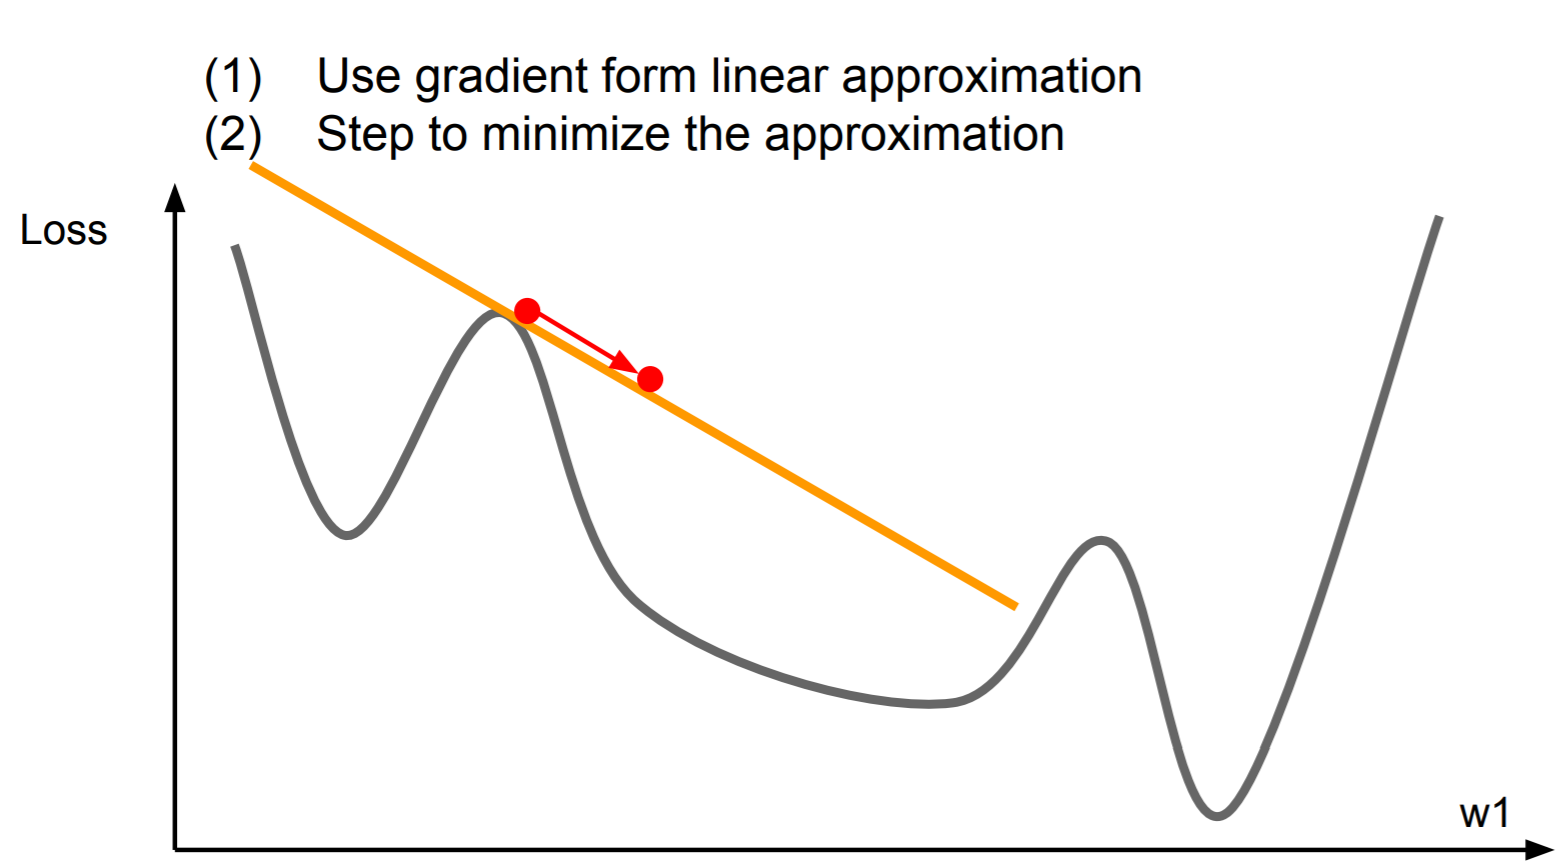
\includegraphics[width=0.7\linewidth]{images/gradient_descent_step.png} 
        \caption{A single step of gradient descent. We form a linear approximation of the loss and step to minimize it.}
    \end{figure}
\end{frame}

\begin{frame}{The Tool: Gradient Descent}
    \framesubtitle{The Update Rule}
    \begin{itemize}
        \item At each step, we update the weights according to the following rule:
        \[
            w^{t+1} = w^{t} - \eta \nabla_{w}J(w^{t})
        \]
        \item Where:
        \begin{itemize}
            \item $w^{t}$ is the vector of weights at step $t$.
            \item $\eta$ (eta) is the \bhighlight{learning rate}, a hyperparameter that controls the step size.
            \item $\nabla_{w}J(w^{t})$ is the gradient of the cost function with respect to the weights.
        \end{itemize}
    \end{itemize}
\end{frame}

\begin{frame}{The Tool: Gradient Descent}
    \framesubtitle{Calculating the Gradient}
    \begin{itemize}
        \item The gradient $\nabla_{w}J$ is computed efficiently using the \bhighlight{backpropagation} algorithm.
        \item Backpropagation is essentially a recursive application of the \bhighlight{chain rule} from calculus to compute the gradient for every parameter in the network.
        \item The process involves two main steps:
        \begin{enumerate}
            \item A \bhighlight{forward pass} to compute the network's output and the final loss.
            \item A \bhighlight{backward pass} to propagate the error gradients from the output layer back to the input layer, calculating the gradient for each weight along the way.
        \end{enumerate}
    \end{itemize}
\end{frame}

\begin{frame}{The Computational Graph}
    \framesubtitle{Why do we need them?}
    \begin{itemize}
        \item As we've seen, the output of a neural network is a deeply nested composite function.
        \item To calculate the gradient of the loss with respect to any weight, we must use the \bhighlight{chain rule} from calculus.
        \item For a network with millions of parameters, applying the chain rule manually is impossible. A \bhighlight{computational graph} is a powerful visualization tool that helps us manage this complexity and automate the process.
    \end{itemize}
\end{frame}

\begin{frame}{The Computational Graph}
    \framesubtitle{Structure}
    \begin{itemize}
        \item A computational graph represents a function as a directed graph:
        \begin{itemize}
            \item \bhighlight{Nodes (Vertices):} Represent operations (e.g., addition, multiplication) or variables.
            \item \bhighlight{Edges:} Represent the flow of data. The output of one node becomes the input to another.
        \end{itemize}
    \end{itemize}
    \begin{figure}
        \centering
        % Source: MLP & Back-prop.pdf, Page: 40
        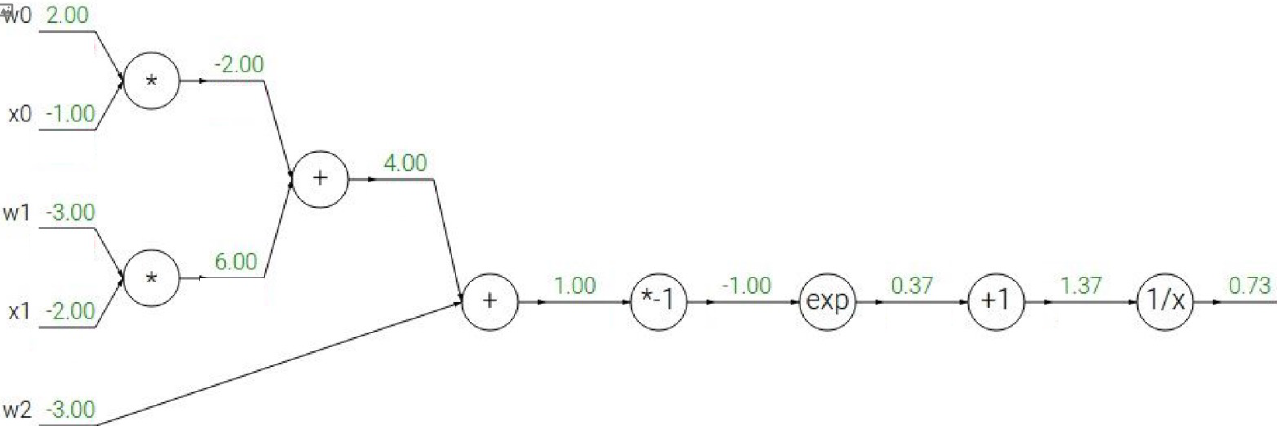
\includegraphics[width=0.9\linewidth]{images/computational_graph_sigmoid_forward.png}
        \caption{A computational graph breaking down a sigmoid neuron into its elementary operations.}
    \end{figure}
\end{frame}

\begin{frame}{The Computational Graph}
    \framesubtitle{The Forward Pass}
    \begin{itemize}
        \item The \bhighlight{forward pass} is the process of evaluating the function represented by the graph.
        \item We start from the input nodes and move forward through the graph, applying the operation at each node to the incoming values.
        \item This continues until we reach the final node, which typically represents the overall loss of the network. The path is determined by the topological sort of the graph's nodes.
    \end{itemize}
    \begin{center}
        \begin{minipage}{0.8\textwidth}
        \begin{figure}
            \centering
            % Source: MLP & Back-prop.pdf, Page: 40
            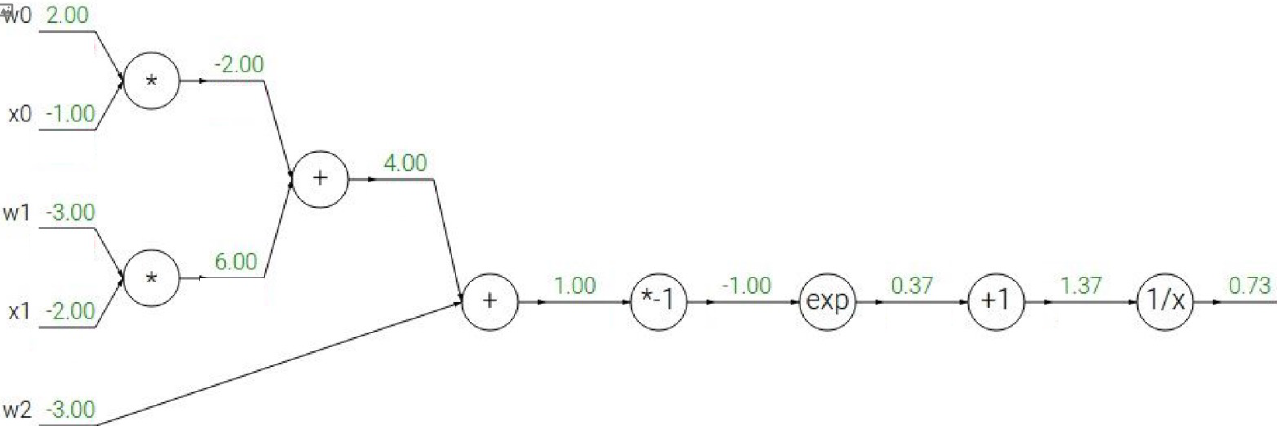
\includegraphics[width=\linewidth]{images/computational_graph_sigmoid_forward.png}
            \caption{In the forward pass, values are computed from left to right. For example, $w_0 \times x_0 = 2.00 \times -1.00 = -2.00$.}
        \end{figure}
        \end{minipage}
    \end{center}
\end{frame}

\begin{frame}{The Computational Graph}
    \framesubtitle{The Backward Pass and The Chain Rule}
    \begin{itemize}
        \item \bhighlight{Backpropagation} is the process of calculating the gradients by moving backward through the graph.
        \item At each node, we use the chain rule to compute the gradient of the final loss with respect to the node's \emph{inputs}, given the gradient with respect to its \emph{output}.
        \item We define three key terms:
        \begin{itemize}
            \item \bhighlight{Upstream Gradient ($\frac{\partial L}{\partial z}$):} The gradient coming from the nodes that follow.
            \item \bhighlight{Local Gradient ($\frac{\partial z}{\partial x}$):} The derivative of the node's operation with respect to its own inputs.
            \item \bhighlight{Downstream Gradient ($\frac{\partial L}{\partial x}$):} The gradient we want to compute and pass backward.
        \end{itemize}
        \[
            \text{Downstream Gradient} = \text{Upstream Gradient} \times \text{Local Gradient}
        \]
    \end{itemize}
\end{frame}

\begin{frame}{The Computational Graph}
    \framesubtitle{Example "Gates"}
    \begin{itemize}
        \item Different nodes (or "gates") distribute the upstream gradient in unique ways based on their local gradient:
    \end{itemize}
    \begin{figure}
        \centering
        % Source: MLP & Back-prop.pdf, Page: 38
        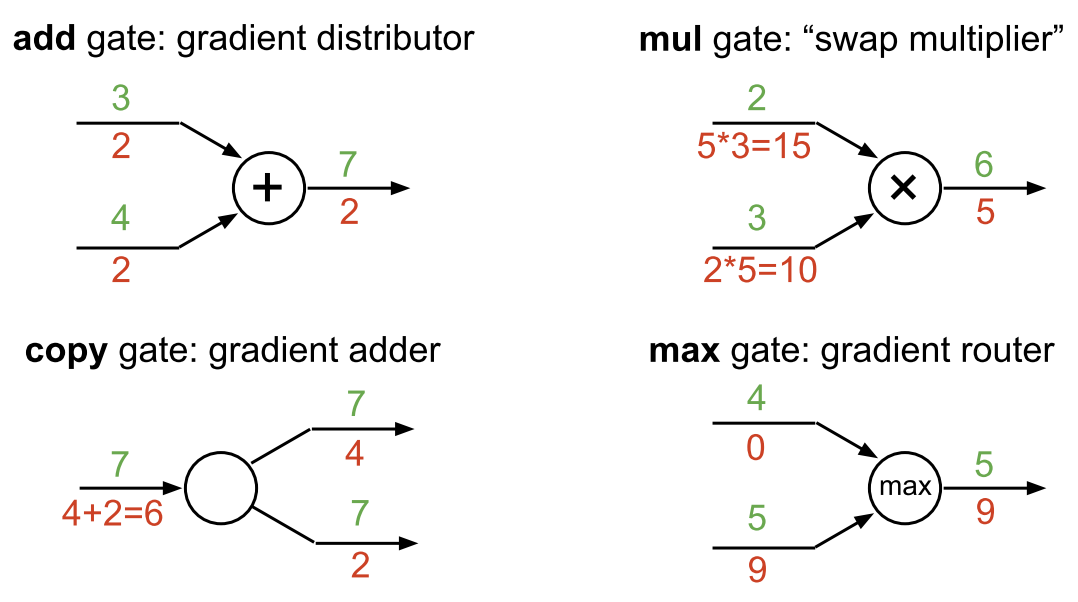
\includegraphics[width=\linewidth]{images/gradient_gates.png}
        \caption{
            \textbf{Add gate:} acts as a "gradient distributor".
            \textbf{Max gate:} acts as a "gradient router".
            \textbf{Multiply gate:} acts as a "swap multiplier".
        }
    \end{figure}
\end{frame}

\begin{frame}{The Computational Graph}
    \framesubtitle{Backpropagation Example: Step 1}
    \begin{itemize}
        \item Let's trace the backward pass for our sigmoid neuron example.
        \item We start at the very end. The gradient of the output with respect to itself is \bhighlight{1}. This is our initial upstream gradient.
    \end{itemize}
    \begin{figure}
        \centering
        % Source: MLP & Back-prop.pdf, Pages: 41-42 (combined view)
        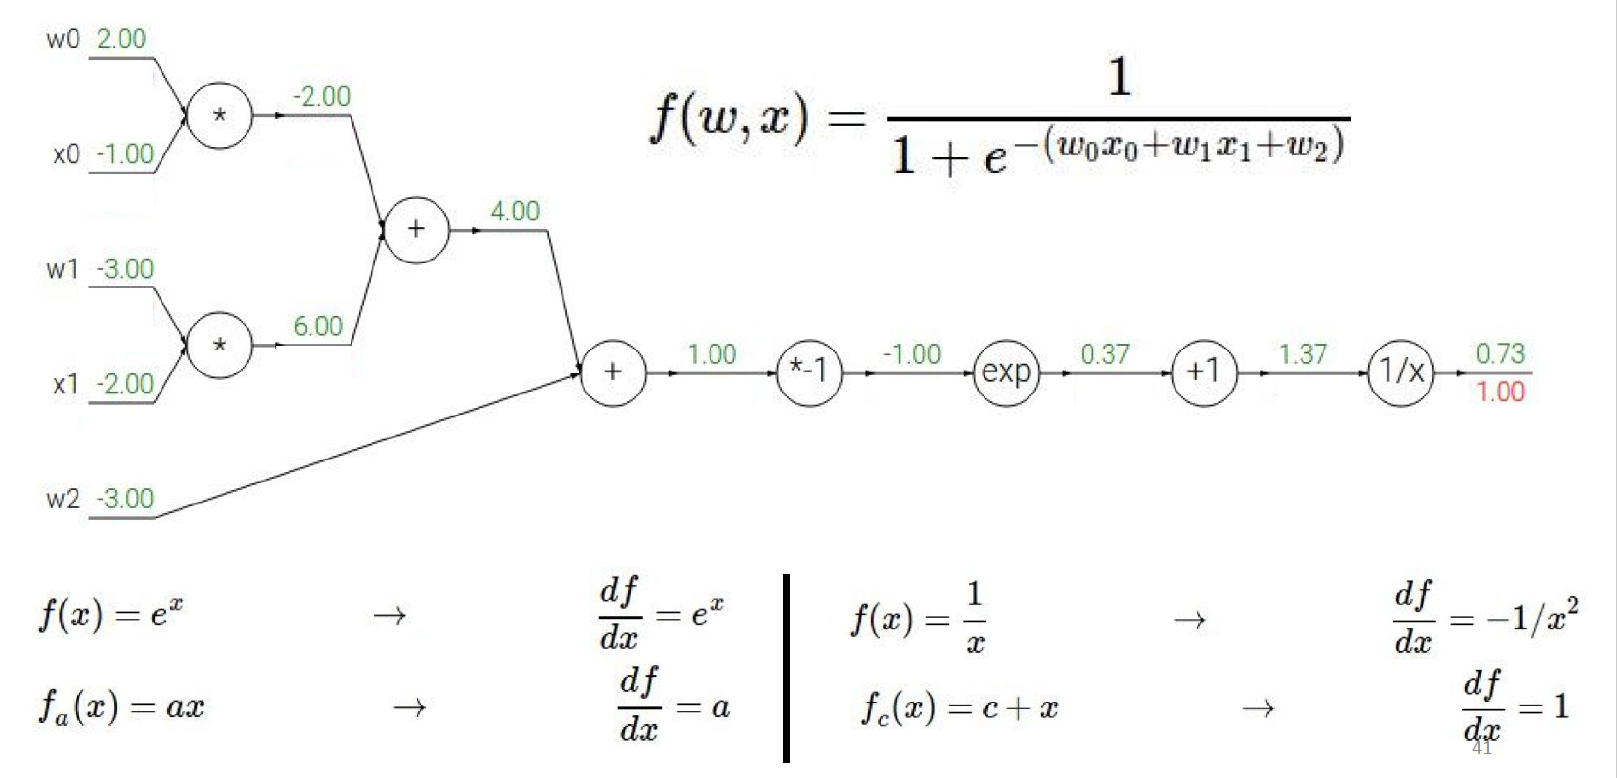
\includegraphics[width=\linewidth]{images/sigmoid_backprop_1.png}
        \caption{Starting the backward pass. The initial gradient at the output is 1.}
    \end{figure}
\end{frame}

\begin{frame}{The Computational Graph}
    \framesubtitle{Backpropagation Example: Step 2}
    \begin{itemize}
        \item The first gate is the $1/x$ gate.
        \item \textbf{Upstream Gradient}: 1.0
        \item \textbf{Local Gradient}: The derivative of $f(x) = 1/x$ is $-1/x^2$. Since the input was 1.37, the local gradient is $-1/(1.37^2) \approx -0.53$.
        \item \textbf{Downstream Gradient}: $1.0 \times -0.53 = -0.53$.
    \end{itemize}
    \begin{figure}
        \centering
        % Source: MLP & Back-prop.pdf, Page: 43
        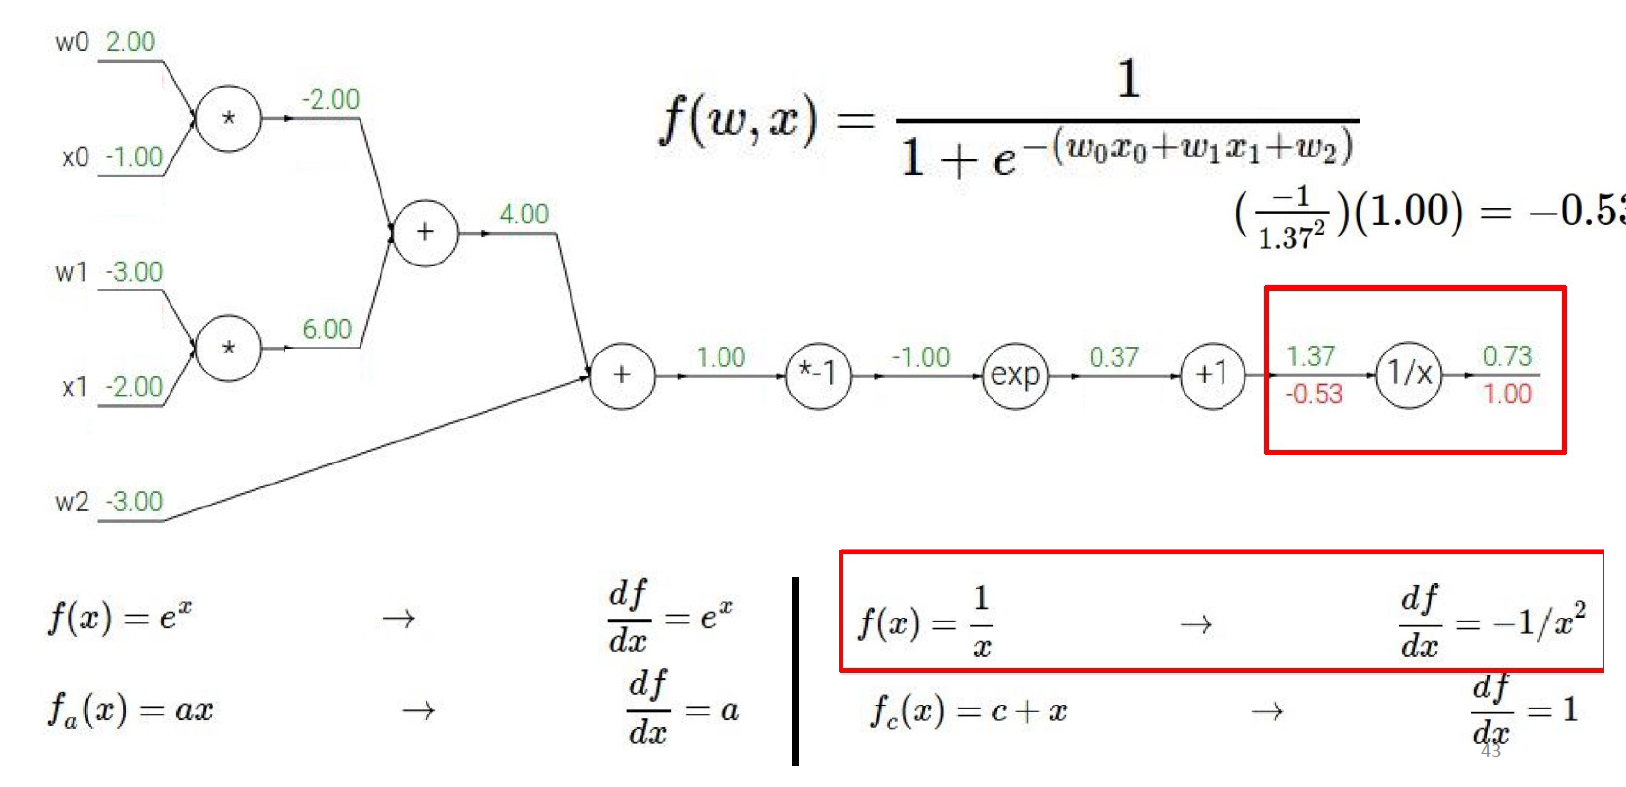
\includegraphics[width=\linewidth]{images/sigmoid_backprop_2.png}
    \end{figure}
\end{frame}

\begin{frame}{The Computational Graph}
    \framesubtitle{Backpropagation Example: Step 3}
    \begin{itemize}
        \item The next gate is the `+1` gate.
        \item \textbf{Upstream Gradient}: -0.53
        \item \textbf{Local Gradient}: The derivative of $f(x) = x+c$ is 1.
        \item \textbf{Downstream Gradient}: $-0.53 \times 1 = -0.53$.
    \end{itemize}
    \begin{figure}
        \centering
        % Source: MLP & Back-prop.pdf, Page: 45
        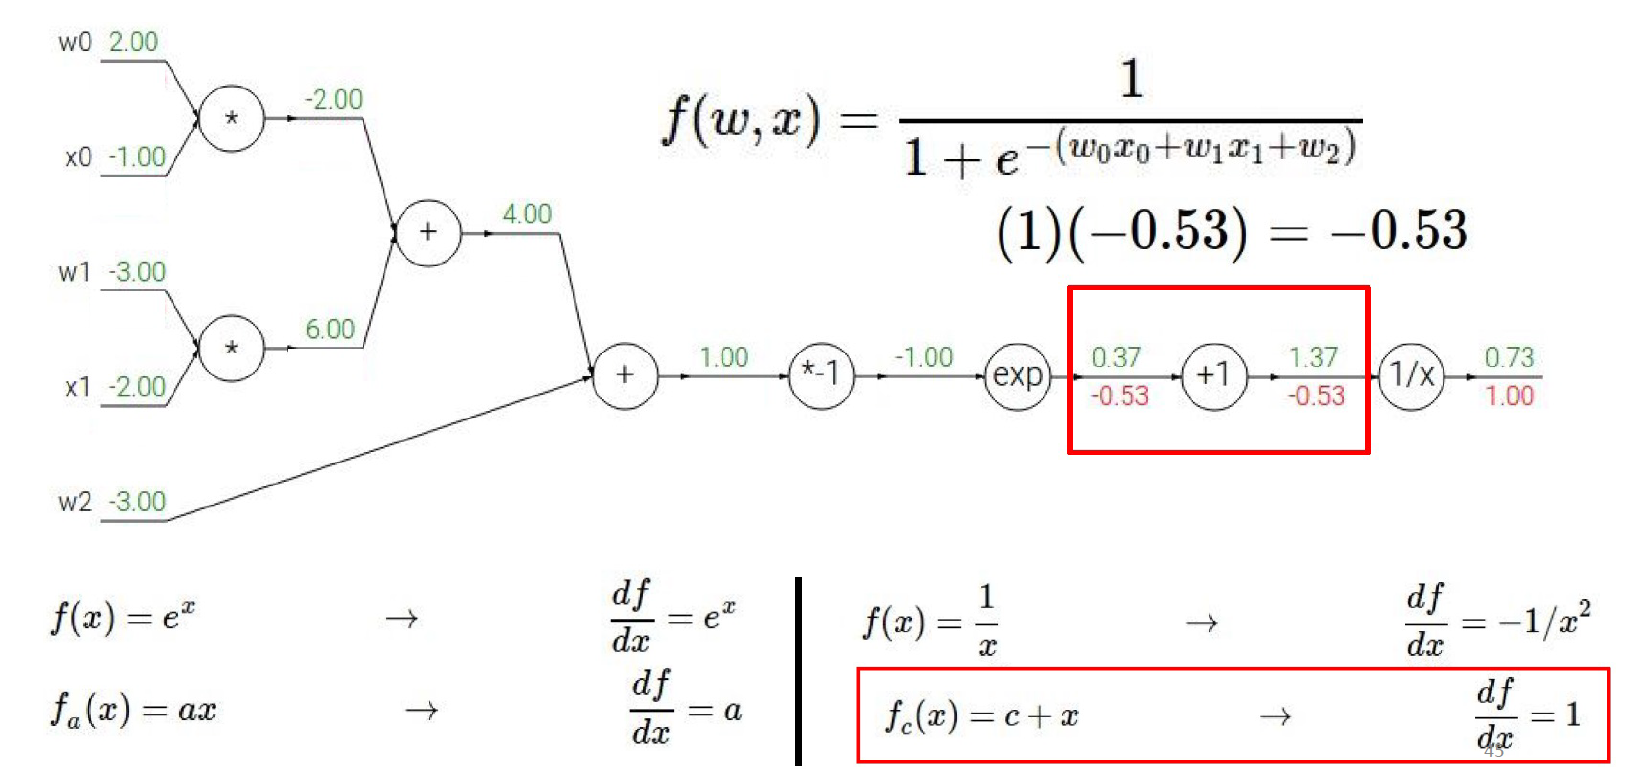
\includegraphics[width=\linewidth]{images/sigmoid_backprop_3.png}
    \end{figure}
\end{frame}

\begin{frame}{The Computational Graph}
    \framesubtitle{Backpropagation Example: Step 4}
    \begin{itemize}
        \item Next is the `exp` gate.
        \item \textbf{Upstream Gradient}: -0.53
        \item \textbf{Local Gradient}: The derivative of $f(x) = e^x$ is $e^x$. Since the input was -1.0, the local gradient is $e^{-1} \approx 0.37$.
        \item \textbf{Downstream Gradient}: $-0.53 \times 0.37 \approx -0.20$.
    \end{itemize}
    \begin{figure}
        \centering
        % Source: MLP & Back-prop.pdf, Page: 48
        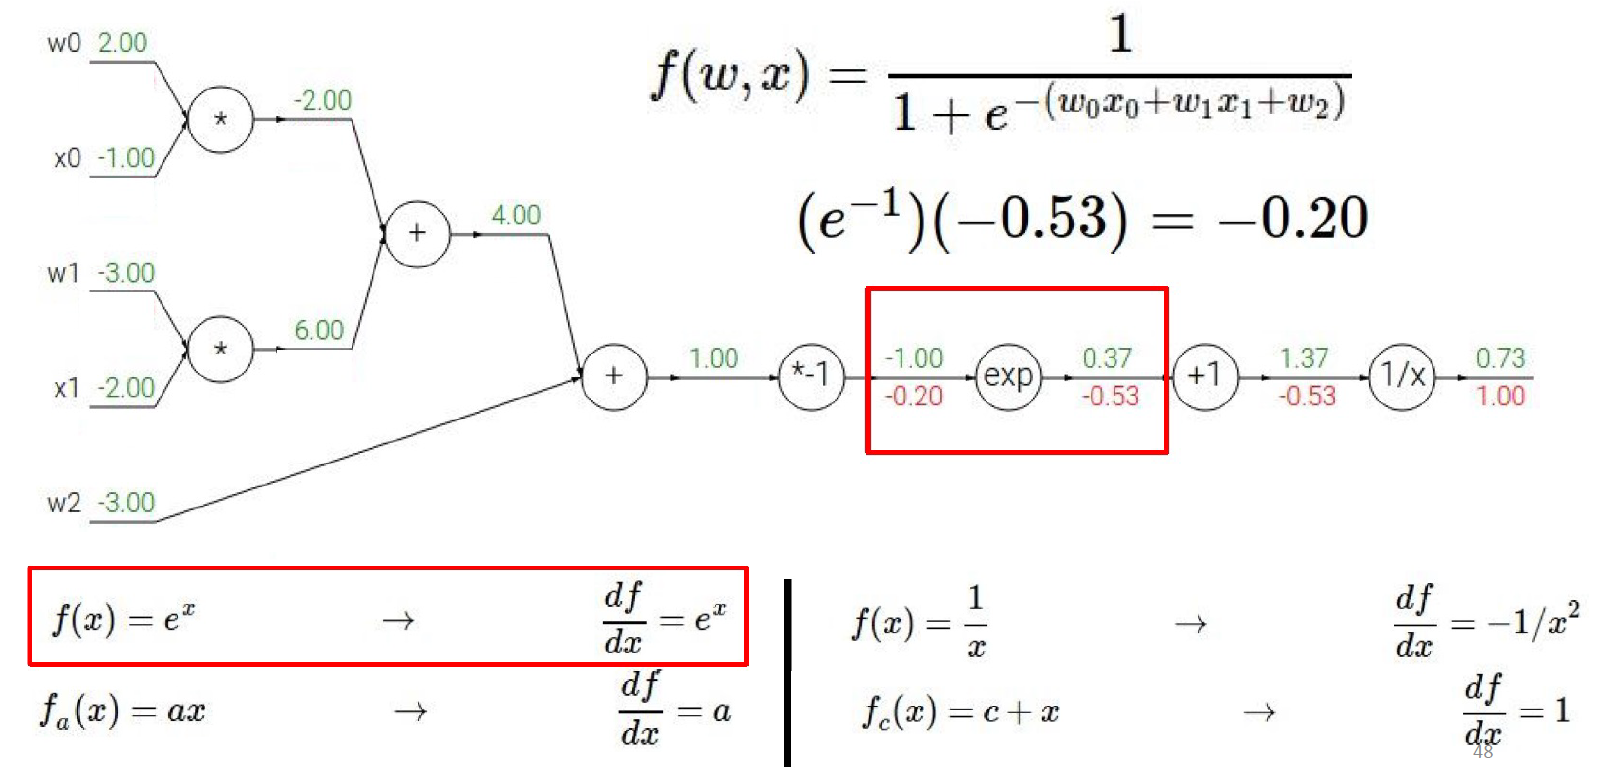
\includegraphics[width=\linewidth]{images/sigmoid_backprop_4.png}
    \end{figure}
\end{frame}

\begin{frame}{The Computational Graph}
    \framesubtitle{Backpropagation Example: Final Steps}
    \begin{itemize}
        \item The gradient is propagated backward through the remaining gates (`*-1`, `+`, `*`).
        \item For example, at the top-most `*` gate (for $w_0, x_0$):
        \begin{itemize}
            \item \textbf{Upstream Gradient}: 0.20 (from the final `+` gate).
            \item \textbf{Local Gradient} for $w_0$: The other input, $x_0 = -1.00$.
            \item \textbf{Downstream Gradient} for $w_0$: $0.20 \times -1.00 = -0.20$.
        \end{itemize}
        \item This process is repeated until we have the gradient for every weight and input.
    \end{itemize}
    \begin{figure}
        \centering
        % Source: MLP & Back-prop.pdf, Page: 53
        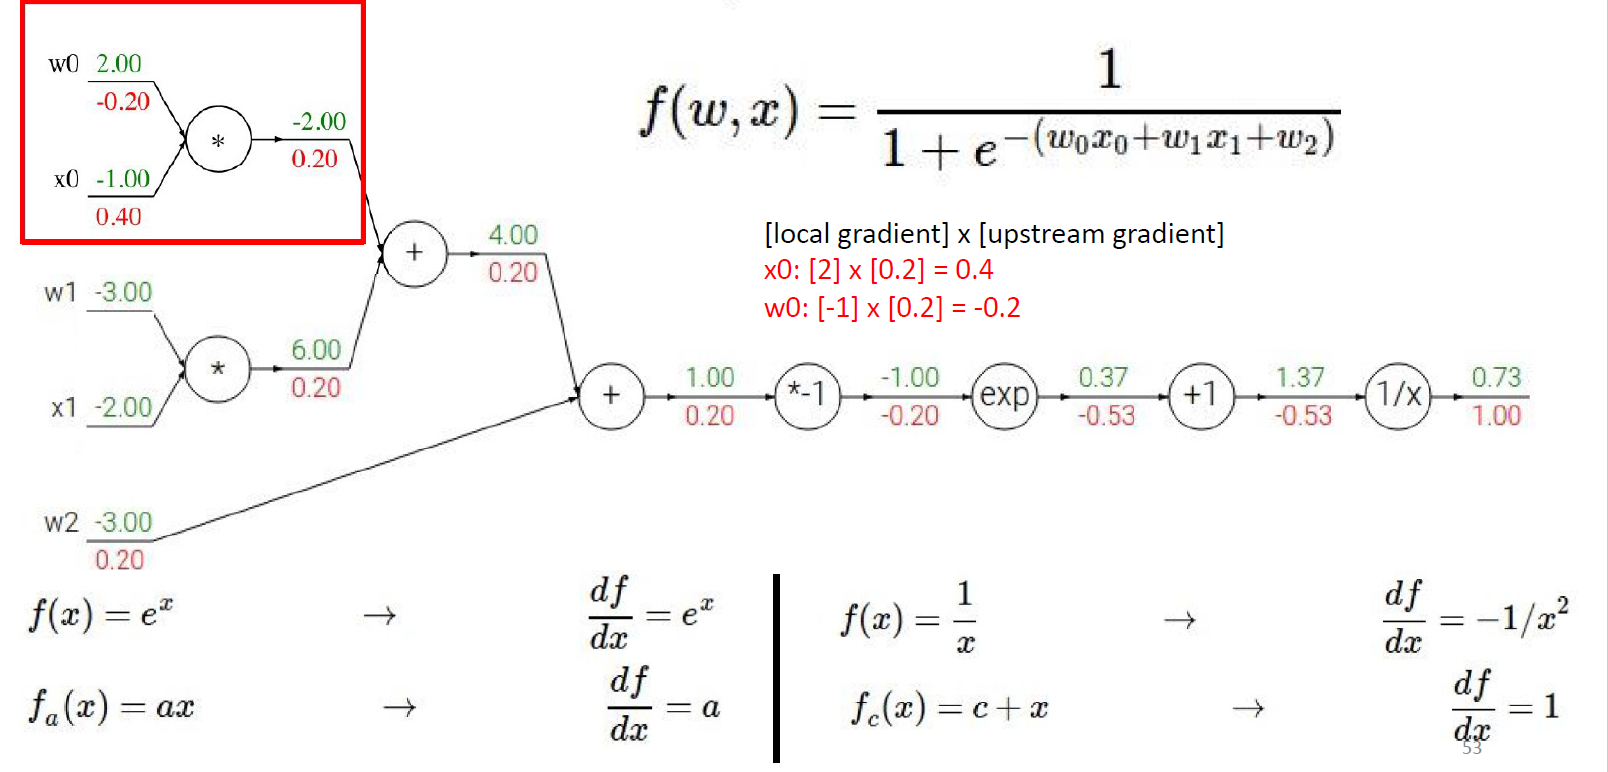
\includegraphics[width=\linewidth]{images/sigmoid_backprop_final.png}
        \caption{The final computed gradients for each weight and input.}
    \end{figure}
\end{frame}

\begin{frame}{From Scalars to Vectors}
    \framesubtitle{Efficient Implementation}
    \begin{itemize}
        \item While the computational graph concept works for single values (scalars), neural networks are implemented using \bhighlight{vectors and matrices} for efficiency.
        \item Instead of calculating gradients one by one, we can process an entire layer or even a mini-batch of data with a few matrix operations.
    \end{itemize}
\end{frame}

\begin{frame}{From Scalars to Vectors}
    \framesubtitle{The Jacobian Matrix}
    \begin{columns}[c]
        \begin{column}{0.5\linewidth}
            \begin{itemize}
                \item The derivative of a vector function with respect to a vector input is a matrix of all possible partial derivatives, called the \bhighlight{Jacobian}.
                \item For a layer's activation $a = f(z)$, the Jacobian $\frac{\partial a}{\partial z}$ tells us how a small change in each input element $z_i$ affects each output element $a_j$.
            \end{itemize}
        \end{column}
        \begin{column}{0.5\linewidth}
            \begin{figure}
                \centering
                % Source: MLP & Back-prop.pdf, Page: 73
                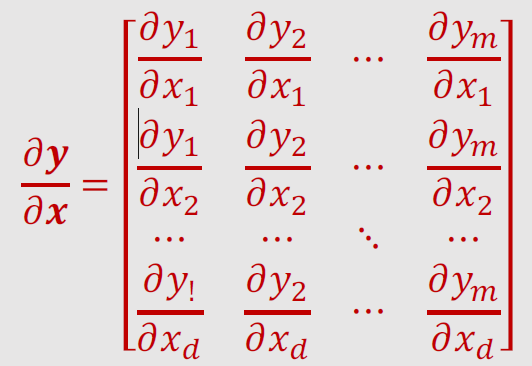
\includegraphics[width=0.8\linewidth]{images/jacobian_matrix.png}
                \caption{Structure of a Jacobian matrix.}
            \end{figure}
        \end{column}
    \end{columns}
\end{frame}

\begin{frame}{From Scalars to Vectors}
    \framesubtitle{Vectorized Forward \& Backward Pass}
    \begin{itemize}
        \item \textbf{Forward Pass:} For a layer $l$, we compute the pre-activation $z^{[l]}$ and activation $a^{[l]}$ for all neurons at once:
        \[ z^{[l]} = W^{[l]}a^{[l-1]} \quad , \quad a^{[l]} = f(z^{[l]}) \]
        \item \textbf{Backward Pass:} We propagate a "sensitivity" or error vector $\delta^{[l]} = \frac{\partial \text{Loss}}{\partial z^{[l]}}$. This vector is passed backward using the chain rule:
        \[ \delta^{[l-1]} = (W^{[l]T}\delta^{[l]}) \odot f'(z^{[l-1]}) \]
        where $\odot$ is element-wise multiplication.
    \end{itemize}
\end{frame}

\begin{frame}{From Scalars to Vectors}
    \framesubtitle{Vectorized Gradient Calculation}
    \begin{itemize}
        \item Once we have the sensitivity vector $\delta^{[l]}$, the gradient for the entire weight matrix of that layer can be computed with a single matrix operation:
        \[ \frac{\partial \text{Loss}}{\partial W^{[l]}} = \delta^{[l]}(a^{[l-1]})^{T} \]
        \item This vectorized approach is significantly more efficient than looping through individual weights.
    \end{itemize}
    \begin{figure}
        \centering
        % Source: MLP & Back-prop.pdf, Page: 63
        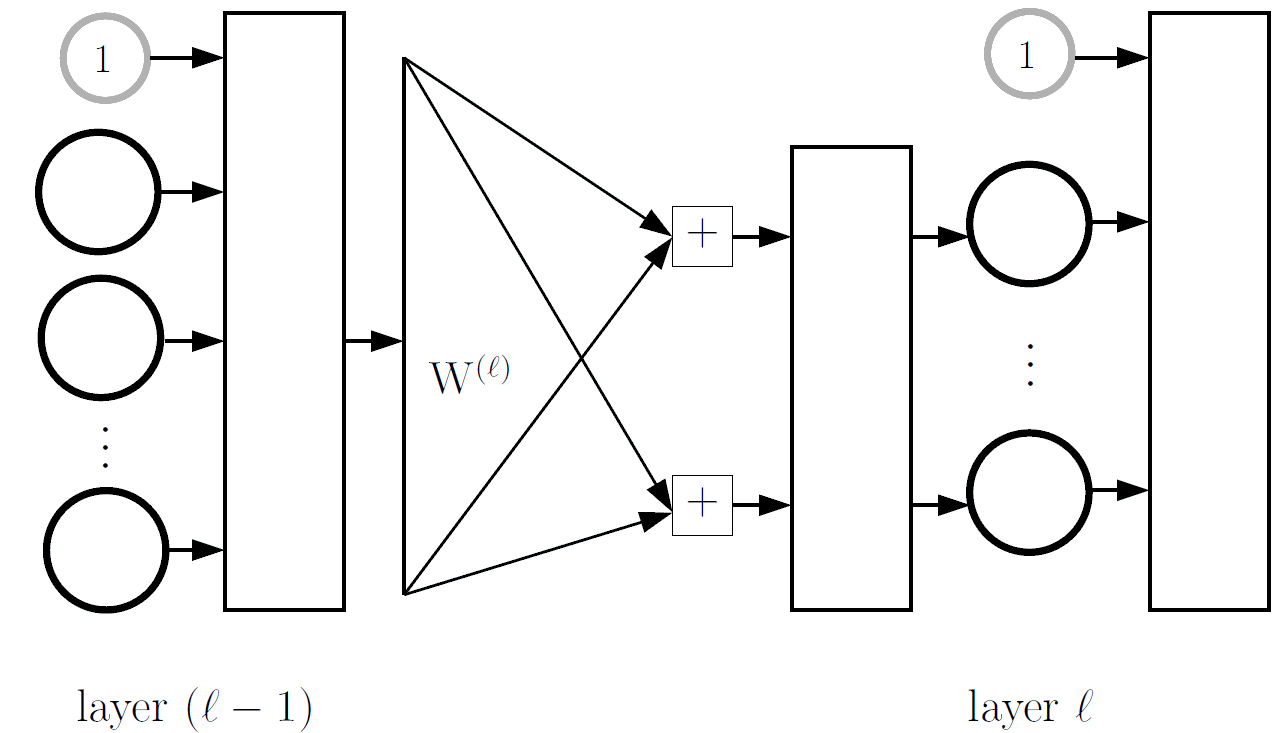
\includegraphics[width=0.8\linewidth]{images/vectorized_backprop.png}
        \caption{Vectorized data flow from the activations of the previous layer ($a^{[l-1]}$) to the current layer ($a^{[l]}$).}
    \end{figure}
\end{frame}

\begin{frame}{The Landscape: Challenges of the Error Surface}
    \begin{itemize}
        \item The error surface for deep networks is complex and \bhighlight{non-convex}, presenting several challenges for gradient descent.
        \item \textbf{Local Minima:} These are points where the gradient is zero, but which are not the global minimum. While a concern, they are less of a problem in high-dimensional spaces than saddle points.
        \item \textbf{Saddle Points:} These are points where the gradient is also zero, but the function curves up in some directions and down in others. Gradient descent can get "stuck" and slow down significantly on them.
    \end{itemize}
    \begin{figure}
        \centering
        % Source: Optimization I.pdf, Page: 3
        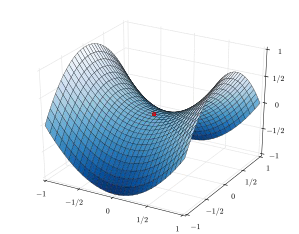
\includegraphics[width=0.4\linewidth]{images/saddle_point.png}
        \caption{A visualization of a saddle point.}
    \end{figure}
\end{frame}

\begin{frame}{The Landscape: Challenges of the Error Surface}
    \framesubtitle{Saddle Points vs. Local Minima}
    \begin{itemize}
        \item A popular and important hypothesis in deep learning is that in large networks, \bhighlight{saddle points are far more common} than local minima.
        \item For a point to be a local minimum, the curvature must be positive in \emph{all} dimensions. For a high-dimensional space, the probability of this is very low.
        \item Therefore, most points with zero gradient that our optimizer finds are likely to be saddle points, not "bad" local minima.
    \end{itemize}
    \begin{figure}
        \centering
        % Source: Optimization I.pdf, Page: 4
        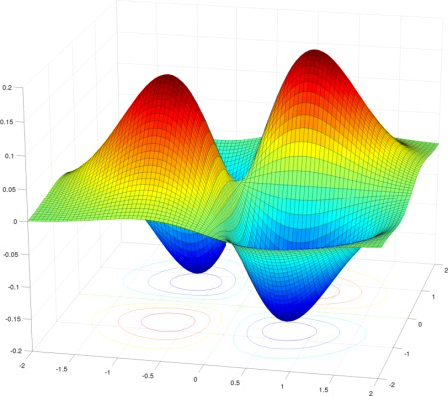
\includegraphics[width=0.5\linewidth]{images/error_surfaces.png}
        \caption{Examples of complex, non-convex error surfaces in neural networks.}
    \end{figure}
\end{frame}

\begin{frame}{Working with Data}
    \framesubtitle{The Problem with Full-Batch Updates}
    \begin{itemize}
        \item In standard (or "batch") gradient descent, we compute the gradient of the cost function using the \bhighlight{entire training dataset} for a single update step.
        \[ \nabla_{w}E(W) = \frac{1}{N} \sum_{n=1}^{N} \nabla_{w}\text{loss}(f(x^{(n)}; W), y^{(n)}) \]
        \item \textbf{The Problem:} For modern datasets with millions of examples, this is extremely slow. We have to process all data just to make one small step.
    \end{itemize}
    \begin{figure}
        \centering
        % Source: Optimization II.pdf, Page: 11
        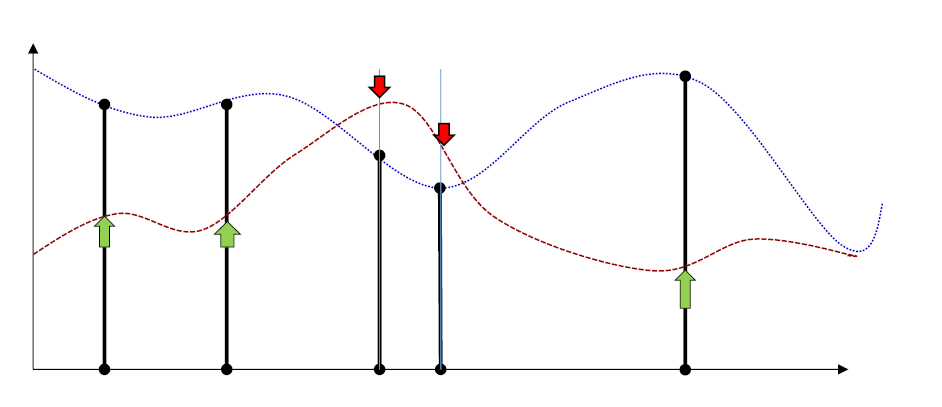
\includegraphics[width=0.7\linewidth]{images/full_batch_idea.png}
        \caption{In batch gradient descent, the algorithm tries to adjust the model based on all training points simultaneously.}
    \end{figure}
\end{frame}

\begin{frame}{Stochastic Gradient Descent (SGD)}
    \framesubtitle{Updating One Sample at a Time}
    \begin{itemize}
        \item The other extreme is \bhighlight{Stochastic Gradient Descent (SGD)}, where we update the weights after seeing \emph{only one} training example at a time.
        \item This makes each update much faster, allowing us to make many more updates in the same amount of time.
    \end{itemize}
    \begin{figure}
        \centering
        % Source: Optimization II.pdf, Page: 15
        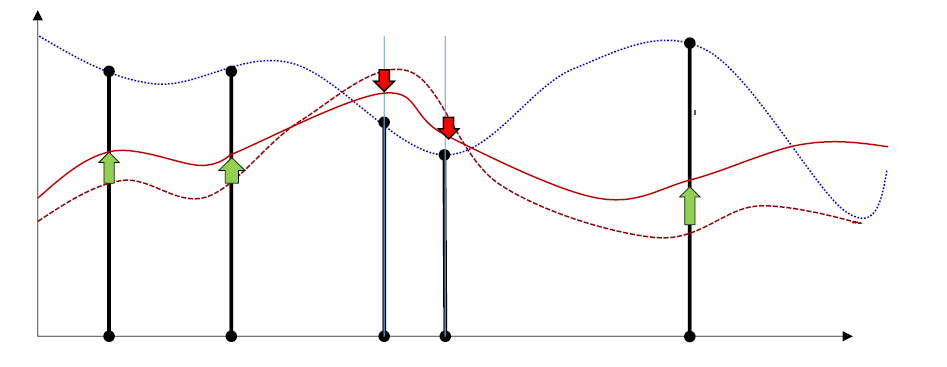
\includegraphics[width=0.7\linewidth]{images/sgd_step_1.png}
        \caption{With SGD, the function is first adjusted for a single, random training point...}
    \end{figure}
\end{frame}

\begin{frame}{Stochastic Gradient Descent (SGD)}
    \framesubtitle{Iterating Through Samples}
    \begin{figure}
        \centering
        % Source: Optimization II.pdf, Page: 16
        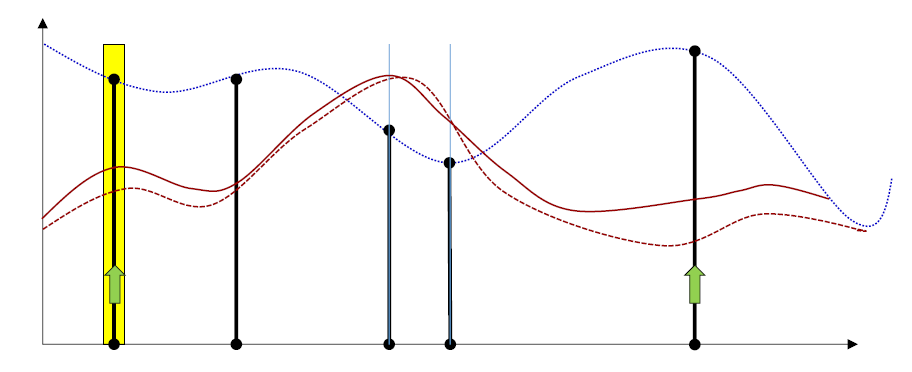
\includegraphics[width=0.7\linewidth]{images/sgd_step_2.png}
        \caption{...then it is adjusted for the next random point...}
    \end{figure}
\end{frame}

\begin{frame}{Stochastic Gradient Descent (SGD)}
    \framesubtitle{Completing an Epoch}
    \begin{figure}
        \centering
        % Source: Optimization II.pdf, Page: 17
        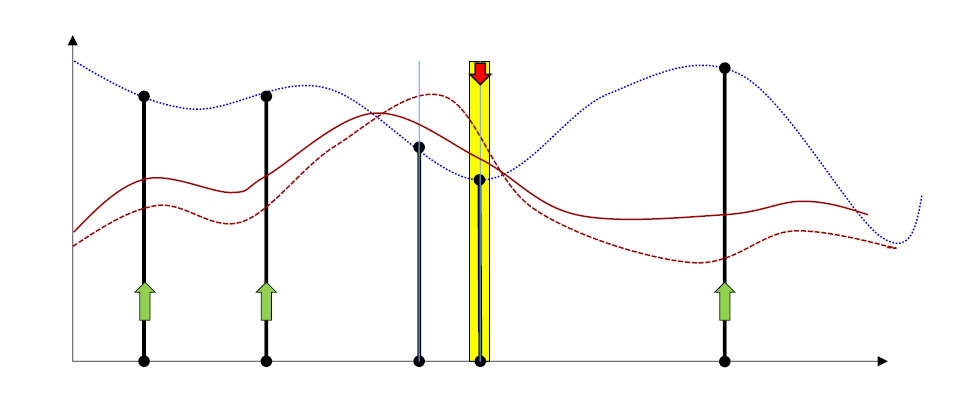
\includegraphics[width=0.7\linewidth]{images/sgd_step_3.png}
        \caption{...and so on. After passing through all points once (an epoch), the entire function has been adjusted.}
    \end{figure}
\end{frame}

\begin{frame}{Stochastic Gradient Descent (SGD)}
    \framesubtitle{The Algorithm and Key Concepts}
    \begin{itemize}
        \item \textbf{The Update Rule:} For a single sample $(x^{(n)}, y^{(n)})$:
        \[ w^{t+1} = w^{t} - \eta \nabla_{w}\text{loss}(f(x^{(n)}; W), y^{(n)}) \]
        \item \textbf{Epoch:} A single full pass through the entire training dataset is called an \bhighlight{epoch}. In one epoch of SGD, we make N weight updates.
        \item \textbf{Crucial Requirement:} For SGD to work correctly, the training data must be \bhighlight{shuffled} at the beginning of every epoch. This randomness is essential for good convergence.
    \end{itemize}
\end{frame}

\begin{frame}{Stochastic Gradient Descent (SGD)}
    \framesubtitle{The "Stochastic" Nature}
    \begin{itemize}
        \item The gradient from a single sample is a "noisy" but \bhighlight{unbiased estimate} of the true gradient over the full dataset.
        \item This high variance means the path to the minimum is erratic and jittery. The updates may not always move towards the minimum and can sometimes move away from it.
    \end{itemize}
    \begin{figure}
        \centering
        % Source: Optimization I.pdf, Page: 9
        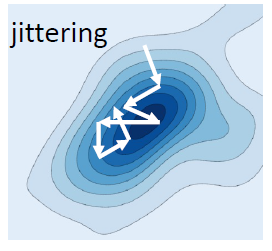
\includegraphics[width=0.2\linewidth]{images/convergence_behaviors.png}
        \caption{The path of SGD often resembles the "jittering" behavior, where it oscillates around the minimum without perfectly converging.}
    \end{figure}
\end{frame}

\begin{frame}{Stochastic Gradient Descent (SGD)}
    \framesubtitle{The Need for Learning Rate Annealing}
    \begin{itemize}
        \item Because the gradient is always noisy, the updates will never settle at the exact minimum if the learning rate $\eta$ remains constant. The optimization will just jitter around it indefinitely.
        \item To ensure convergence, the learning rate must be \bhighlight{decayed over time}. This is called \bhighlight{learning rate annealing} or scheduling.
        \item A common strategy is to start with a relatively high learning rate for fast initial progress and gradually reduce it to allow for fine-tuning near the minimum.
    \end{itemize}
\end{frame}

\begin{frame}{Mini-Batch Gradient Descent}
    \framesubtitle{The Best of Both Worlds}
    \begin{itemize}
        \item \bhighlight{Mini-Batch Gradient Descent} is the standard method used in practice. It's a compromise between the full-batch and SGD approaches.
        \item We compute the gradient on a small, random subset of the data called a \bhighlight{mini-batch}.
    \end{itemize}
    \begin{figure}
        \centering
        % Source: Optimization II.pdf, Page: 24
        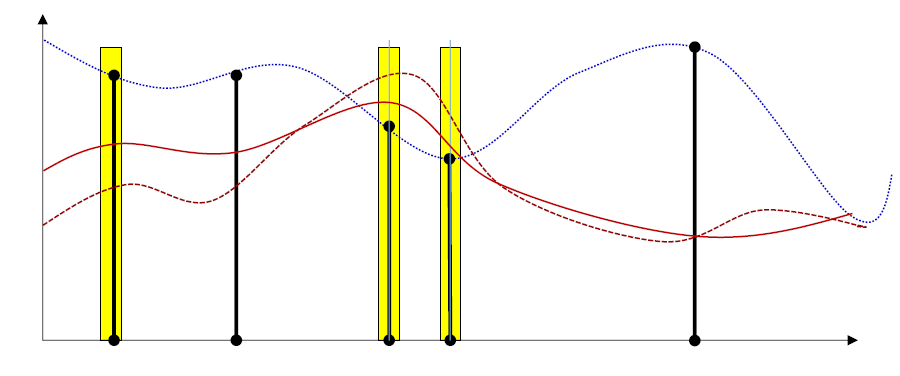
\includegraphics[width=0.7\linewidth]{images/minibatch_idea.png}
        \caption{In Mini-Batch GD, we update the model based on a small, random subset of the data.}
    \end{figure}
\end{frame}

\begin{frame}{Mini-Batch Gradient Descent}
    \framesubtitle{Advantages}
    \begin{itemize}
        \item \textbf{Efficiency:} It allows us to take advantage of the massive parallelization capabilities of GPUs. Matrix operations on a mini-batch are much more efficient than processing samples one by one.
        \item \textbf{Stability:} By averaging gradients over a small batch, we reduce the variance of the updates, leading to a more stable convergence than pure SGD. The path towards the minimum is less erratic.
    \end{itemize}
\end{frame}

\begin{frame}{Comparing the Update Strategies}
    \framesubtitle{A Visual Guide}
    \begin{figure}
        \centering
        % Source: Optimization II.pdf, Page: 47
        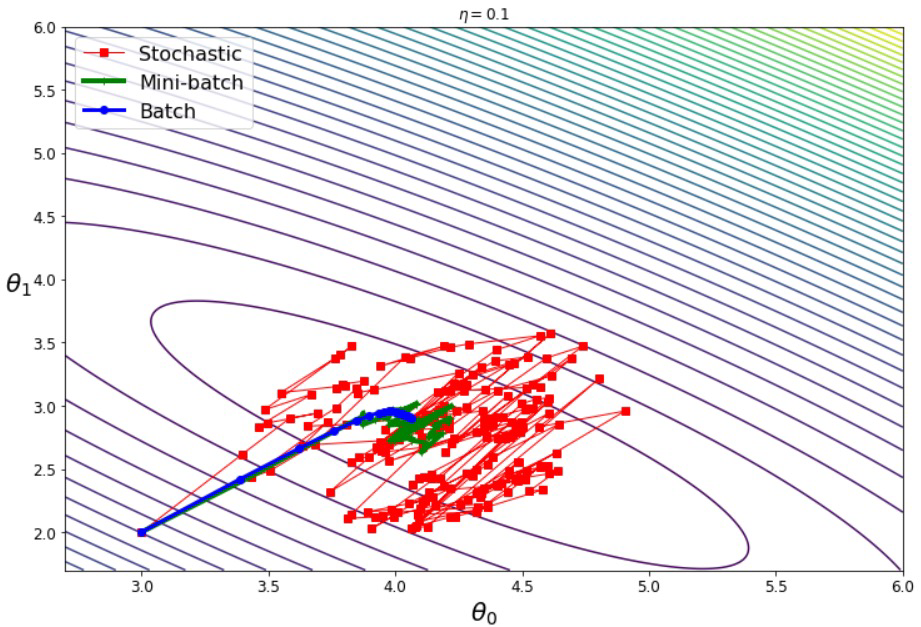
\includegraphics[width=0.9\linewidth]{images/optimizer_paths.png}
        \caption{
            \textbf{Batch (Blue):} Takes a smooth, direct path but each step is very slow.
            \textbf{Stochastic (Red):} Very noisy and erratic path, but takes many fast steps.
            \textbf{Mini-Batch (Green):} A good balance, reducing noise while still being computationally efficient.
        }
    \end{figure}
\end{frame}

\begin{frame}{Choosing the Mini-Batch Size}
    \framesubtitle{A Practical Guideline}
    \begin{itemize}
        \item The mini-batch size is a hyperparameter that needs to be chosen.
        \item If the training set is very small (e.g., < 2000 examples), you can often use full-batch gradient descent.
        \item For larger datasets, typical mini-batch sizes are powers of 2, such as \bhighlight{32, 64, 128, 256, 512}.
        \item A key constraint is that the mini-batch of data and the resulting gradients must fit into your GPU's memory.
    \end{itemize}
\end{frame}

\begin{frame}{Regularization: Dropout}
    \framesubtitle{A Simple and Powerful Idea}
    \small
    \begin{itemize}
        \item \bhighlight{Dropout} is a regularization technique that prevents complex co-adaptations on training data by randomly dropping units (along with their connections) from the neural network during training.
        \item \textbf{The Core Idea:} In each forward pass, for each training example, we randomly set the output of some neurons to zero.
        \item The probability of keeping a neuron active is a hyperparameter, often set to 0.5.
    \end{itemize}
    \begin{figure}
        \centering
        % Source: Regularization.pdf, Page: 24
        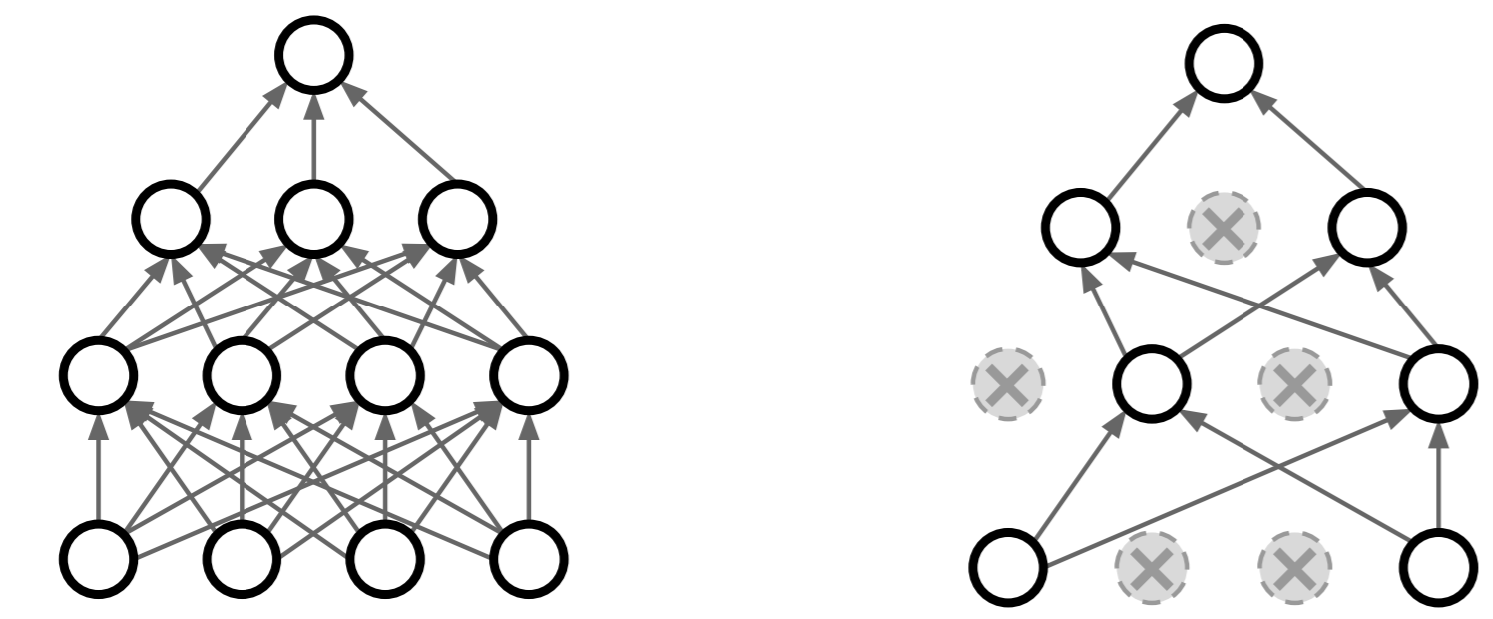
\includegraphics[width=0.7\linewidth]{images/dropout_idea.png}
        \caption{Left: A standard neural network. Right: The same network after applying dropout. Some neurons are temporarily deactivated.}
    \end{figure}
\end{frame}

\begin{frame}{Dropout: The Training Process}
    \framesubtitle{Training a Thinned Network}
    \small
    \begin{itemize}
        \item During each training step, we are effectively training a different, "thinned" version of the network for each mini-batch.
        \item The backpropagation step only updates the weights of the "active" neurons and connections for that specific forward pass.
        \item This forces the network to learn more robust and redundant features, as it cannot rely on any single neuron to be present.
    \end{itemize}
    \begin{figure}
        \centering
        % Source: Regularization.pdf, Page: 31
        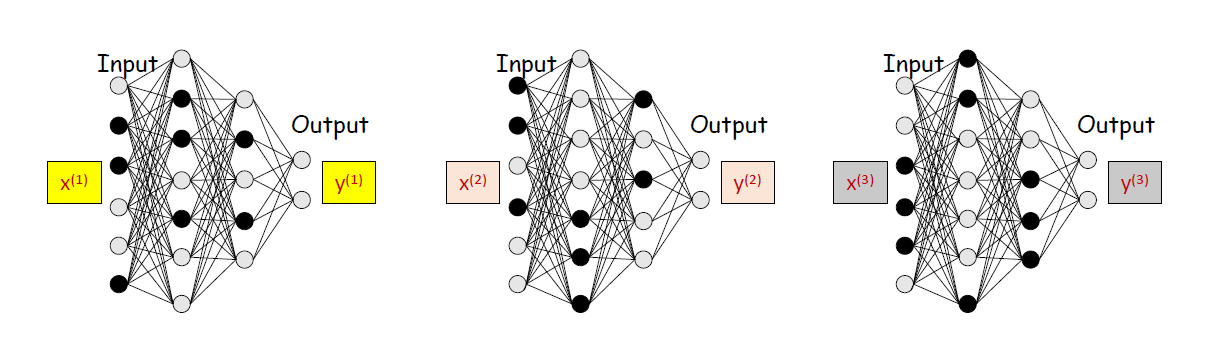
\includegraphics[width=\linewidth]{images/dropout_training_process.png}
        \caption{For each training example, a different random subset of neurons is deactivated, creating a unique "thinned" network.}
    \end{figure}
\end{frame}

\begin{frame}{Why Does Dropout Work?}
    \framesubtitle{Intuition 1: Preventing Co-adaptation}
    \small 
    \begin{itemize}
        \item Dropout prevents neurons from \bhighlight{co-adapting} too much.
        \item A neuron cannot rely on the presence of other specific neurons to correct its mistakes, because those other neurons might be dropped out at any time.
        \item Therefore, each neuron is forced to learn features that are useful on their own, leading to more robust and independent representations.
    \end{itemize}
    \begin{figure}
        \centering
        % Source: Regularization.pdf, Page: 29
        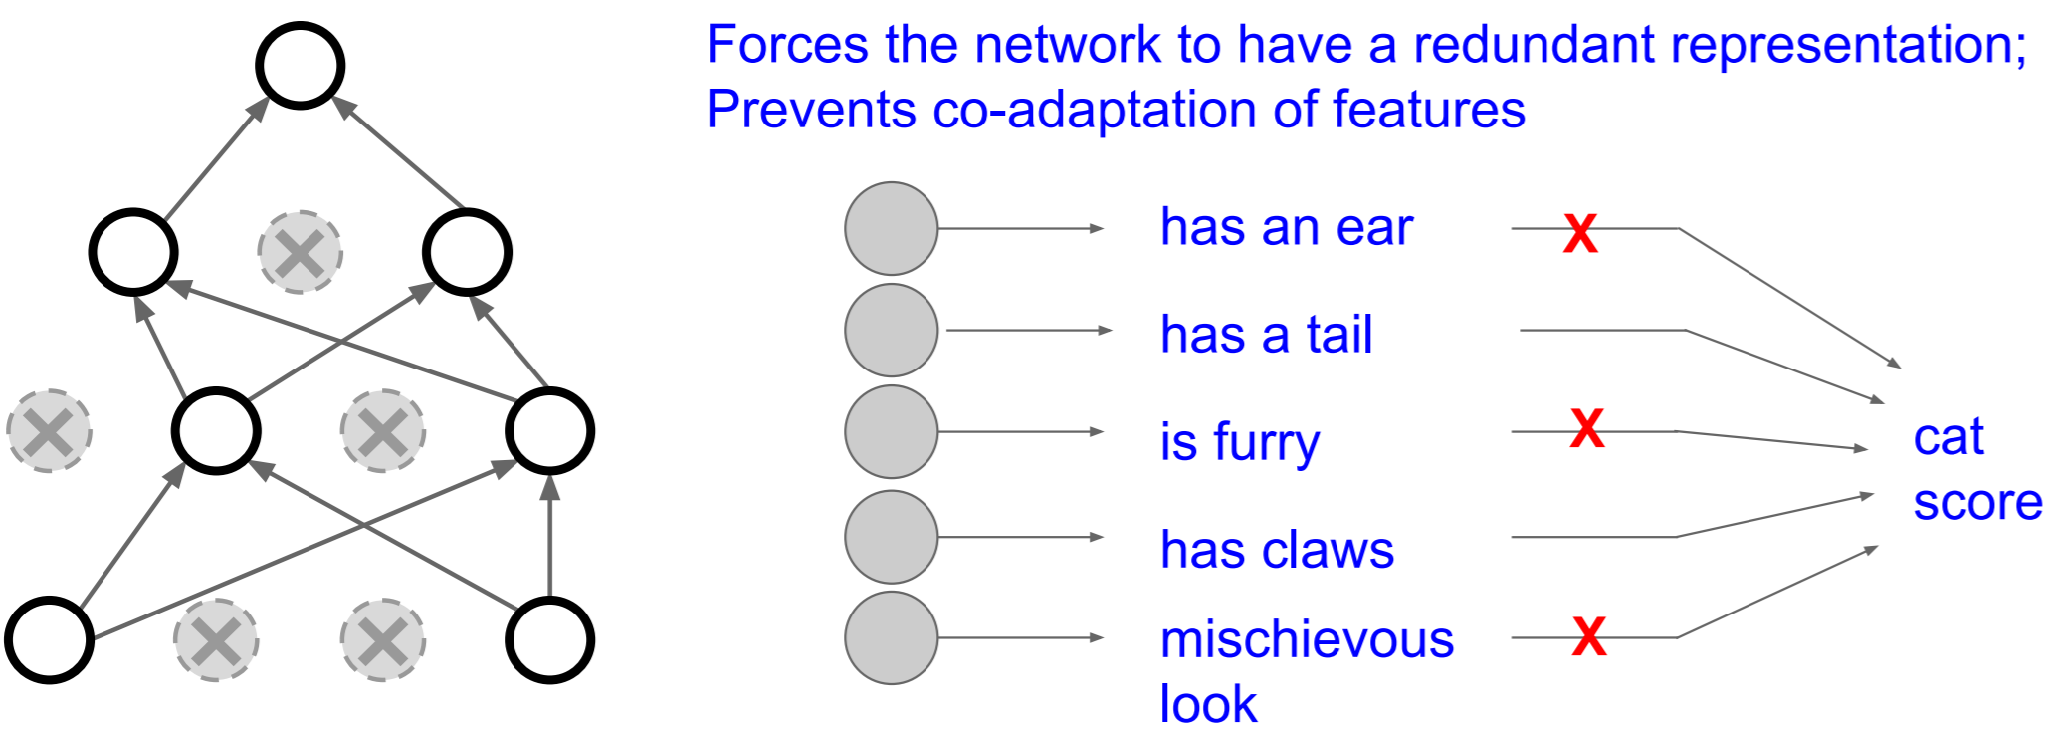
\includegraphics[width=0.8\linewidth]{images/dropout_coadaptation.png}
        \caption{Without dropout, a neuron might learn to rely on a specific feature (e.g., "has whiskers"). With dropout, it must learn from a more diverse set of features.}
    \end{figure}
\end{frame}

\begin{frame}{Why Does Dropout Work?}
    \framesubtitle{Intuition 2: An Ensemble of Networks}
    \small 
    \begin{itemize}
        \item Dropout can be viewed as an efficient way of training a huge \bhighlight{ensemble} of different neural networks.
        \item Each time we randomly drop out neurons, we are essentially training a different network architecture. For a network with N neurons, there are $2^N$ possible thinned networks!
        \item All these networks share weights, so we are effectively training an exponentially large number of models in parallel. At test time, we want to average their predictions.
    \end{itemize}
    \begin{figure}
        \centering
        % Source: Regularization.pdf, Page: 34
        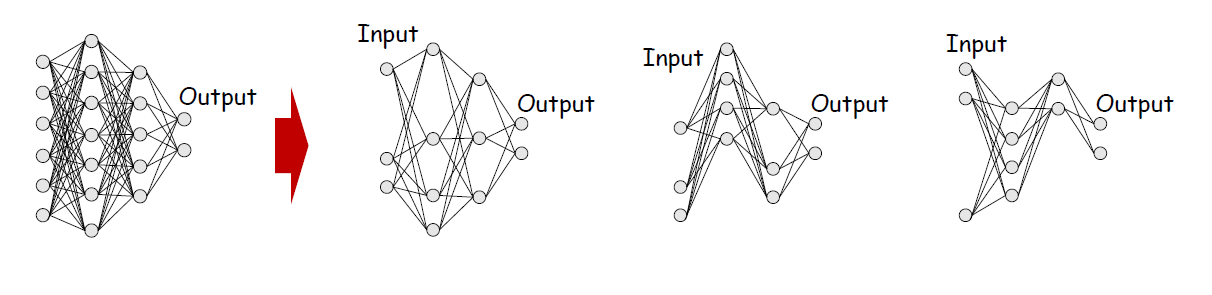
\includegraphics[width=\linewidth]{images/dropout_ensemble.png}
        \caption{Each dropout mask corresponds to training a different sub-network, but they all share the same underlying weights.}
    \end{figure}
\end{frame}

% --- SLIDE WITH CORRECTION ---
\begin{frame}{Dropout at Test Time}
    \framesubtitle{The Problem of Randomness}
    \begin{itemize}
        \item We cannot have random outputs at test time. We need a single, deterministic prediction.
        \item The ideal solution would be to average the predictions of all $2^N$ possible sub-networks, but this is computationally impossible.
        \item \textbf{A Simple Solution:} At test time, we use the full network with all neurons active, but we \bhighlight{scale down the weights} by the probability $p$ (the keep probability) that a neuron was active during training.
        \[ W_{\text{test}} = p \times W_{\text{train}} \]
    \end{itemize}
\end{frame}

\begin{frame}{Inverted Dropout}
    \framesubtitle{A More Common Implementation}
    \begin{itemize}
        \item A more common and practical method is \bhighlight{Inverted Dropout}.
        \item The key idea is to perform the scaling during \bhighlight{training time} instead of test time.
        \item During the forward pass of training, after dropping neurons, the activations of the remaining neurons are immediately scaled up by dividing by the keep probability $p$.
        \[ a^{[l]}_{\text{train}} = \frac{a^{[l]}_{\text{train}} * \text{mask}}{p} \]
        \item \textbf{Advantage:} The forward pass at test time remains completely unchanged. We don't need to do any extra scaling or modifications. This is much cleaner to implement.
    \end{itemize}
\end{frame}

\begin{frame}{Dropout: Practical Considerations}
    \framesubtitle{Tips and Trade-offs}
    \begin{itemize}
        \item \textbf{When to use it:} If your network is significantly overfitting, Dropout is a very effective regularizer.
        \item \textbf{Training Time:} Training with dropout typically takes longer to converge because the gradient updates are noisier and each neuron is trained less often.
        \item \textbf{Dropout Strength:} The keep probability $p$ (often between 0.5 and 0.8) is a hyperparameter you need to tune. A lower $p$ means stronger regularization.
        \item \textbf{Interaction with Batch Norm:} Some evidence suggests that Batch Normalization can reduce the need for Dropout. Using both might not always provide additional benefits.
    \end{itemize}
\end{frame}

\begin{frame}{Dropout: Typical Results}
    \framesubtitle{Impact on Generalization}
    \begin{figure}
        \centering
        % Source: Regularization.pdf, Page: 47
        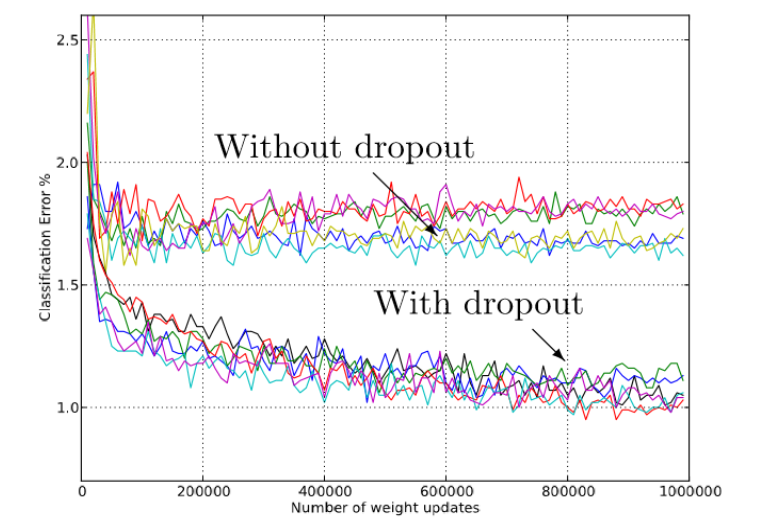
\includegraphics[width=0.9\linewidth]{images/dropout_results.png}
        \caption{A typical result showing that a network trained \textbf{with dropout} (bottom curves) achieves a lower classification error on the test set compared to the same network trained \textbf{without dropout} (top curves).}
    \end{figure}
\end{frame}

\begin{frame}{Generalization: Data Augmentation}
    \framesubtitle{The Best Regularizer: More Data}
    \begin{itemize}
        \item One of the most effective ways to improve a model's generalization is simply to train it on more data.
        \item However, collecting and labeling new data can be expensive and time-consuming.
        \item \bhighlight{Data Augmentation} is a powerful technique to artificially expand the training dataset by creating modified, yet realistic, copies of existing data.
    \end{itemize}
\end{frame}

\begin{frame}{Data Augmentation}
    \framesubtitle{The Core Idea}
    \begin{itemize}
        \item The core idea is to apply transformations to an input example in a way that \bhighlight{does not change its label}.
        \item For example, a horizontally flipped image of a cat is still an image of a cat.
        \item This teaches the model to become \bhighlight{invariant} to these transformations, helping it focus on the true underlying features of the class rather than irrelevant variations in the input.
    \end{itemize}
\end{frame}

\begin{frame}{Data Augmentation}
    \framesubtitle{Examples for Image Data}
    \begin{figure}
        \centering
        % Source: Regularization.pdf, Page: 49
        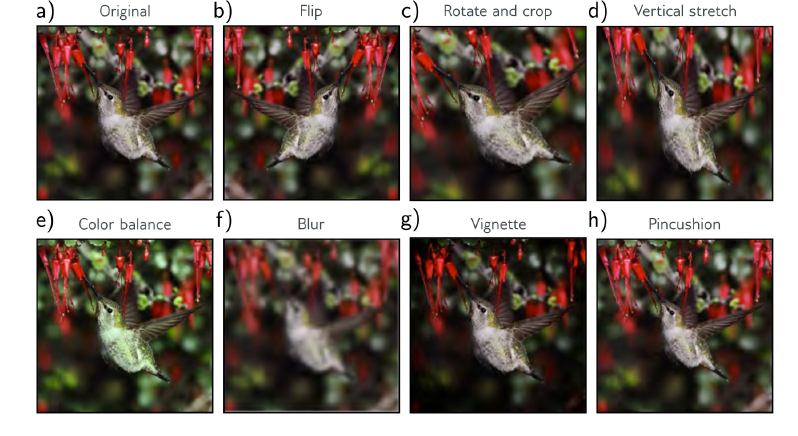
\includegraphics[width=\linewidth]{images/data_augmentation_examples.png}
        \caption{Common augmentation techniques for images include flipping, rotating, cropping, color shifting, blurring, and adding distortions.}
    \end{figure}
\end{frame}

\begin{frame}{Data Augmentation}
    \framesubtitle{Another Technique: Adding Noise}
    \begin{itemize}
        \item Another form of data augmentation is to add random noise directly to the input data.
        \item This can make the model more robust and less sensitive to small variations in the input, effectively acting as a regularizer.
    \end{itemize}
    \begin{figure}
        \centering
        % Source: Regularization.pdf, Page: 51
        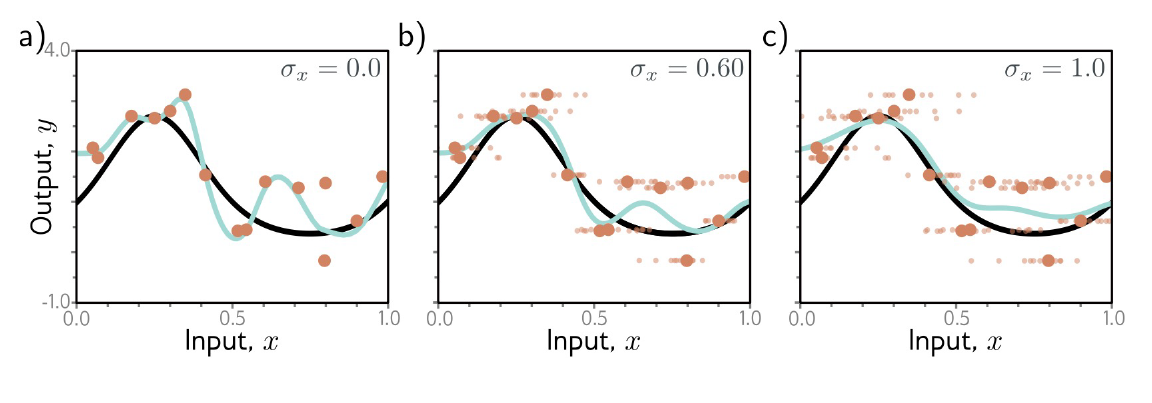
\includegraphics[width=0.8\linewidth]{images/augmentation_noise.png}
        \caption{The effect of adding increasing levels of noise ($\sigma_x$) to the input data during training.}
    \end{figure}
\end{frame}




\end{document}